%----------------------------------------------------------------------------------------
%	Capítulo 1
%----------------------------------------------------------------------------------------
\newpage
\clearpage{\pagestyle{empty}\cleardoublepage}
\doublespacing
\newpage
%% NUEVO CAPITULO X
\chapter{Marco problemático}
\pagestyle{myportland}
\pagenumbering{arabic}
\newpage



%% NUEVA SECCIÓN X.X
\section{Definición de la problemática}

Actualmente, la crianza de o cultivo de truchas en el Perú se da de manera artesanal, los procesos involucrados son realizados por operarios. La automatización de procesos manuales aumenta diversos factores que van desde la calidad del producto hasta la capacidad de producción. \textbf{Una empresa nacional} ubicada en la \textbf{región de Lima} se dedica a la producción, venta y distribución de trucha arcoíris de diversos gramajes que se comercializan en el mercado nacional. Dicha empresa nacional realizó una \textbf{consultoría privada} el año 2018, detectó altos porcentajes de mortandad y desaparición de truchas\footnote{Cerca del 20\% que representan aproximadamente 18 000 truchas.} en la etapa de engorde\footnote{17.5 centímetros en adelante.}.

Según la consultoría, \textbf{la mortandad} y \textbf{desaparición de las truchas en la etapa de engorde} se debe a la alta densidad de las truchas en las jaulas flotantes. Las principales causas de un alto grado de desaparición están asociadas enfermedades y a la característica carnívora de las truchas, es decir, pueden alimentarse de otras truchas. \textbf{Las truchas deben ser clasificadas periódicamente} en sus respectivas jaulas flotantes, según tallas. Sin embargo, debido a la complejidad y cantidad de esfuerzo manual requerido\footnote{Cuatro operarios para una jaula de 3 $ m^3 $ que contienen 5000 truchas requieren 50 $ h $.}, la clasificación no es muy frecuente. Además, realizar el proceso de forma manual estresa a la trucha, pudiendo causar una muerte por estrés. Debido a esto, \textbf{el presente trabajo busca automatizar dicho proceso}.

%% NUEVO SUBSECCION X.X.X
\subsection{Justificación}

Según la empresa nacional, reducir la mortandad en el cultivo artesanal de truchas aumentará la capacidad de producción. Se detalla que cuando dichas truchas atraviesan las etapas de \textit{alevinos III} (7.5 a 10.0 cm.), \textit{juvenil I} (10.0 a 13.5 cm.) y \textit{engorde} (17 cm. en adelante) aumenta la mortandad respecto a las otras etapas, siendo engorde la que más importancia tiene. La clasificación y conteo manual puede agravarse ya que en tiempos de mayor presencia fluvial se realiza el trabajo bajo condiciones meteorológicas adversas que dificultan el trabajo haciéndolo más lento y en oportunidades inviable debido a que se requiere el uso de generadores de electricidad, hacer uso de estos en esas condiciones puede generar accidentes. 

Este trabajo de investigación aborda desde la problemática hasta el diseño conceptual que servirá como punto de partida para el diseño y posterior implementación de la máquina y sistemas que la compongan.

%% NUEVO SUBSECCION X.X.X
\subsection{Alcance}

Este trabajo busca diseñar un sistema clasificador y contador de truchas arcoíris de un determinado rango de tamaños. Así mismo, se busca integrar nuevas tecnologías y mé-todos, según sean viabilidad técnica y económica, al diseño conceptual.

%% NUEVO SUBSECCION X.X.X
\subsection{Objetivos}

Se presenta el objetivo general y los objetivos específicos del presente trabajo.

%% NUEVA SUB-SUB-SECCION X.X.X.X
\subsubsection{Objetivo general}

Realizar el diseño conceptual de un sistema clasificador y contador de truchas arcoíris de 15 a 20 centímetros.

%% NUEVA SUB-SUB-SECCION X.X.X.X
\subsubsection{Objetivos específicos}

\begin{itemize}
\item Definir la problemática: identificar procesos críticos en la crianza artesanal de trucha arcoíris y seleccionar un proceso.
\item Elaborar el diseño conceptual: elaborar la lista de exigencias, estructura de funciones, matriz morfológica y plantear tres conceptos de solución.
\item Seleccionar la solución óptima y elaborar el diagrama de operaciones de la so-lución óptima. 
\end{itemize}

%% NUEVO SUBSECCION X.X.X
\subsection{Metodología}

La metodología, que contempla las recomendaciones para encontrar una solución óptima, está basada en el libro \textit{Engineering Design – A Systematic Approach}.\footnote{Traducción: \textit{"Diseño de ingeniería: un enfoque sistemático"}}  Esta metodología puede incluir múltiples normas de diseño, en este caso las normas VDI 2221-2225 \textit{(La Asociación de Ingenieros Alemanes)}.

El análisis, el términos generales, consiste en recopilar información, realizar una lista de requerimientos, discernir entre procesos críticos que pueden ser automatizados, separar los procesos en sistemas que cumplan funciones, listar las mejores opciones para cada subsistema, iterar hasta encontrar la solución más óptima que integre todos los subsistemas, proponer tres o más soluciones óptimas como concepto de solución, seleccionar una de estas y realizar su diagrama de operaciones .

%% NUEVA SECCIÓN X.X
\section{Estado del arte}
\textbf{El estado del arte es una categoría central y deductiva que se aborda y propone como estrategia un análisis crítico} de las dimensiones políticas, epistemológicas y pedagógicas de la producción investigativa en la evaluación de aprendizaje.\citep{GuevaraPatino2016} \textbf{El aspecto técnico del estado del arte, al que se hace referencia en este estudio, se basa en el desarrollo de una investigación técnica documental y técnica de campo.} La técnica documental permite la selección de información para explicar las teorías que sustentan el estudio de los fenómenos y procesos.\citep{Martinez2003} Además, las técnicas de investigación de campo son aquellas que el investigador utiliza en el desarrollo práctico o teórico de su proceso investigativo con el fin de corroborar sus objetivos generales y específicos.\citep{GuevaraPatino2016}

%% NUEVO SUBSECCION X.X.X
\subsection{Crianza de truchas}

%% NUEVA SUB-SUB-SECCION X.X.X.X
\subsubsection{Nacional}
En el Perú, el \textbf{cultivo de trucha se da predominantemente de forma manual} ya que el sector es dirigido por pequeñas y medianas empresas. La capacidad de producción del Perú es alta debido a la gran cantidad de especies, recursos hidrobiológicos\footnote{Se refieren a los organismos que pasan toda su vida o parte de ella en un ambiente acuático y son utilizados por el hombre de forma directa o indirecta.\citep{MINAGRI2011}} y climas.

\textbf{El gobierno peruano implementó medidas} para impulsar su desarrollo mediante el MEF\footnote{Ministerio de Economía y Finanzas.}  en el marco de estrategia de Gobierno de impulsar y promocionar los sectores con alto potencial productivo. \textbf{Las medidas acuícolas se centran en seis ejes}: primero, fortalecimiento de la Autoridad Sanitaria; segundo, una regulación que garantice el cumplimiento de estándares de sanidad, inocuidad, ambientales y de calidad de los productos; tercero, escalar y abrir nuevos mercados para las exportaciones acuícolas; cuarto, impulsar la gestión y articulación interinstitucional; quinto, promocionar apoyo tecnológico e innovación en especial para las micro y pequeñas empresas; sexto, mejorar infraestructura. \citep{Andina2019}

\begin{figure}[H]
	\centering
	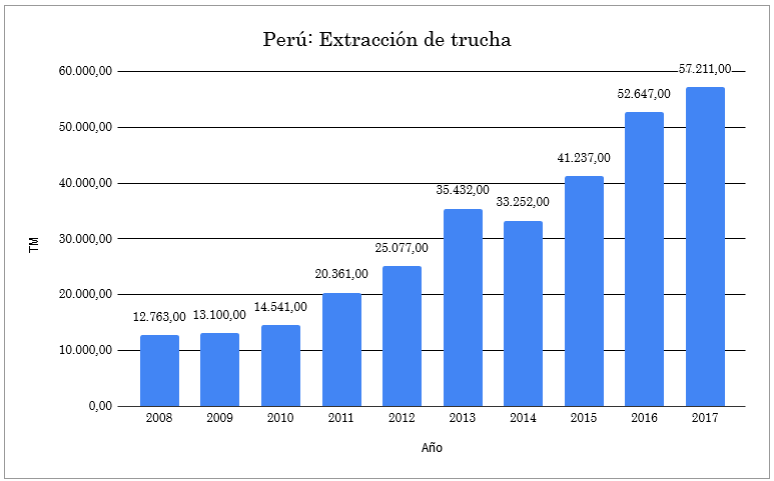
\includegraphics[width=1\textwidth]{chapter1/extraccion trucha toneladas anuales.png}
	\caption{Extracción de trucha en toneladas métricas anuales.}
	 Datos: \citep{MinisteriodelaProducciondelPeru2018} 	 \\ 
	 Gráfico: Elaboración propia.
	\label{fig:Extracción de trucha en toneladas métricas anuales}
\end{figure}

%% NUEVA SUB-SUB-SECCION X.X.X.X
\subsubsection{Internacional}

En \textbf{China}\footnote{Asia concentra alrededor del 90\% de la acuicultura mundial.\citep{Powell2003}}, principal país exportador en acuicultura a nivel mundial con 20 mil millones de dólares \citep[p.~44]{FAO2017}, se usa métodos de crianza de truchas que reducen la \textit{mortandad} y el \textit{estrés hídrico} que afectan a las truchas. Procesos automatizados y estandarizados aumentaron la producción de trucha arcoíris a nivel internacional. Lograron una reducción importante de costos en el cultivo debido a la automatización. Se controla la calidad de agua, contaminación por exceso de excremento de las truchas, temperatura del agua, tasa de crecimiento, etc. \citep[p.~1-6]{2017}

En \textbf{Japón}, segundo país que más importa productos pesqueros a nivel mundial \citep[p.~44]{FAO2017}, produce alrededor de 50000 especies de peces, lo que representa aproximadamente 10 mil toneladas anuales. La crianza de truchas se da en estanques de agua corriente, en lagunas y en aguas marinas profundas (estanques con agua de mar bombeadas desde la profundidad del océano 100 m. o más). Sin embargo, nuevas invasiones de patógenos están mermando la producción y debido a esto se crearon fármacos. La industria se encuentra altamente industrializada. \citep[p.~1-5]{2005} 

En el inciso \textbf{\ref{ssec:productos comerciales y patentes}} se muestran productos y patentes de origen internacional, desarrollados para el sector acuícola y que son cercanos al estudio en este trabajo.

\begin{table}[H]
	\centering	
	\caption{Comercio internacional de productos pesqueros por principales importadores y exportadores en miles de dólares.}
	\label{tbl:comercio internacional de productos pesqueros por principales importadores y exportadores en dolares}
	\begin{tabular}{ l }
		\begin{minipage}{1\textwidth}
			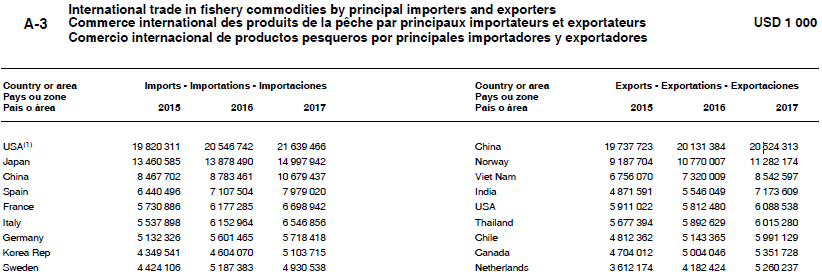
\includegraphics[width=1\textwidth]{chapter1/comercio internacional de productos pesqueros por principales importadores y exportadores en dolares.png}
		\end{minipage}	
	\end{tabular}
	\\	Fuente: FAO.
\end{table}

%% NUEVO SUBSECCION X.X.X
\subsection{Sistema de clasificación de peces}
\label{ssec:sistema de clasificacion de peces}

Existen \textbf{dos dimensiones} en las que se basa la clasificación: \textbf{la distancia desde la boca hasta la aleta caudal} en sus respectivos extremos y \textbf{la circunferencia} que alrededor del pez cerca del inicio de la aleta dorsal. En la Figura \ref{fig:anatomia de la trucha arcoiris} se muestra la anatomía de la especie y se puede observar las regiones de la trucha.

En la práctica, sabiendo que se puede aproximar una medida a partir de la otra, solo se toma la distancia que cubre las tres regiones.\footnote{La toma de datos de manera manual suele ser hasta 100 veces más lenta que otros métodos.} Se realiza este proceso para evitar problemas que afecten negativamente la producción: truchas en competencia por alimento, aumento de diferencia en tallas, reducción del rendimiento del alimento, aumento de mortandad en los peces de menor talla, disminución de calidad y talla. Con una clasificación adecuada y oportuna se trata de \textbf{prevenir el canibalismo}\footnote{Las truchas son carnívoras por lo que pueden alimentarse de su misma especie, en este caso de los de menor talla.}, uniformizar el crecimiento para brindar una alimentación adecuada a la talla, prevenir estrés y agotamiento de los peces.\citep[p.~16]{Flores2010} 

\begin{figure}[H]
	\centering
	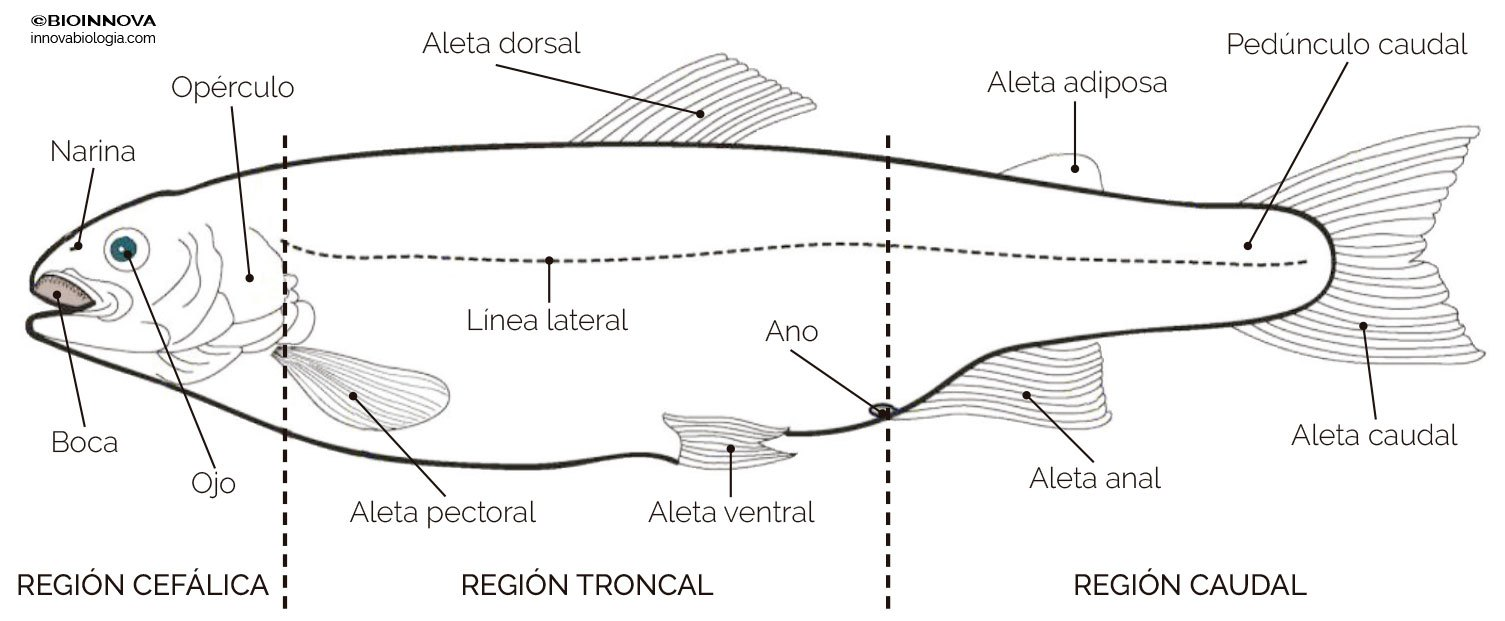
\includegraphics[width=1\textwidth]{chapter1/anatomia de la trucha arcoiris.png}
	\caption{Anatomía de la trucha arcoíris \textit{(Oncorhynchus mykiss)}.}
	Fuente: Bioinnova.
	\label{fig:anatomia de la trucha arcoiris}
\end{figure}


La clasificación por tamaño permite identificar en qué etapa de producción se encuentra la trucha. Identificar las etapas permite brindar un plan de alimentación adecuado y reducir la sobre-alimentación. En la Tabla \ref{tbl:clasificacion de truchas por etapas de produccion} se muestra las etapas existentes según FONDEPES\footnote{Fondo Nacional de Desarrollo Pesquero}.

% Please add the following required packages to your document preamble:
% \usepackage[table,xcdraw]{xcolor}
% If you use beamer only pass "xcolor=table" option, i.e. \documentclass[xcolor=table]{beamer}
\begin{table}[H]
	\centering	
	\caption{Clasificación de truchas por etapas de producción.}
	\label{tbl:clasificacion de truchas por etapas de produccion}
	\begin{tabular}{l|c|c|c|c|c|c|c|c|c|}
		\cline{2-10}
		& \cellcolor[HTML]{9B9B9B}{\color[HTML]{000000} \textbf{\rot{Siembra}}} & \cellcolor[HTML]{9B9B9B}{\color[HTML]{000000} \textbf{\rot{Alevinaje I}}} & \cellcolor[HTML]{9B9B9B}{\color[HTML]{000000} \textbf{\rot{Alevinaje II}}} & \cellcolor[HTML]{9B9B9B}{\color[HTML]{000000} \textbf{\rot{Alevinaje III}}} & \cellcolor[HTML]{9B9B9B}{\color[HTML]{000000} \textbf{\rot{Juvenil I}}} & \cellcolor[HTML]{9B9B9B}{\color[HTML]{000000} \textbf{\rot{Juvenil II}}} & \cellcolor[HTML]{9B9B9B}{\color[HTML]{000000} \textbf{\rot{Engorde I}}} & \cellcolor[HTML]{9B9B9B}{\color[HTML]{000000} \textbf{\rot{Engorde II}}} & \cellcolor[HTML]{9B9B9B}{\color[HTML]{000000} \textbf{\rot{Cosecha}}} \\ \hline
		\multicolumn{1}{|l|}{\cellcolor[HTML]{9B9B9B}\textbf{De \textit{(mm)}}} & - & 35 & 51 & 81 & 121 & 141 & 171 & 201 & 261 \\ \hline
		\multicolumn{1}{|l|}{\cellcolor[HTML]{9B9B9B}\textbf{Hasta \textit{(mm)}}} & 34 & 50 & 80 & 120 & 140 & 170 & 200 & 260 & - \\ \hline
		\multicolumn{1}{|l|}{\cellcolor[HTML]{9B9B9B}\textbf{De \textit{(g)}}} & - & 2.81 & 6.91 & 11 & 51 & 110 & 153 & 200 & 251 \\ \hline
		\multicolumn{1}{|l|}{\cellcolor[HTML]{9B9B9B}\textbf{Hasta \textit{(g)}}} & 2.80 & 6.90 & 10 & 50 & 109 & 152 & 199 & 250 & 290 \\ \hline
		\multicolumn{1}{|l|}{\cellcolor[HTML]{9B9B9B}\textbf{Este trabajo \textit{(mm)}}} & \multicolumn{3}{c|}{} & \multicolumn{4}{c|}{\cellcolor[HTML]{C0C0C0}100 a 200} & \multicolumn{2}{c|}{} \\ \hline
	\end{tabular}
	\\Fuente: FONDEPES.
\end{table}

%% NUEVA SUB-SUB-SECCION X.X.X.X
\subsubsection{Clasificación manual}

La clasificación manual se \textbf{recomienda cuando la cantidad de truchas no supera las 1000 truchas}.\citep[p.~25]{FAO2014} Las cajas clasificadoras ya sean de anchura fija o ajustables son fabricadas artesanalmente como las mostradas en la Figura \ref{fig:clasificadora de anchura fija rejillas de clasificacion y clasificadora ajustable} Estas cajas de madera y metal con barras de metal o compuestos montados en su base dejan pasar por las rejillas a los peces que tienen determinada circunferencia, es decir, se realiza una clasificación por forma.\citep[p.~15]{FAO2005}

\begin{figure}[H]
	\centering
	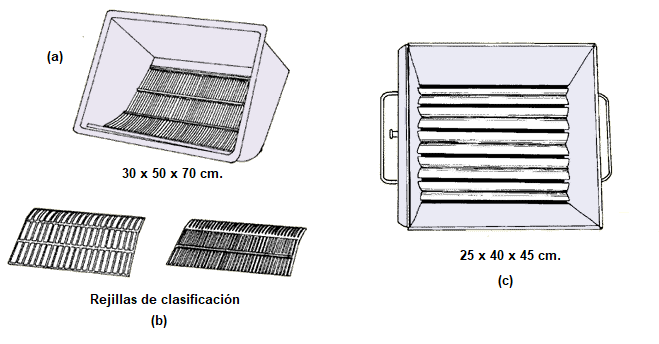
\includegraphics[width=1\textwidth]{chapter1/clasificadora de anchura fija rejillas de clasificacion y clasificadora ajustable.png}
	\caption{(a,b,c) Clasificadora de anchura fija, rejillas de clasificación y clasificadora ajustable.}
	Fuente: FAO.
	\label{fig:clasificadora de anchura fija rejillas de clasificacion y clasificadora ajustable}
\end{figure}

Para realizar el proceso de clasificación manual (Figura \ref{fig:clasificacion y medicion manual de truchas}) se siguen tareas consecutivas: limpiar la caja clasificadora, preparar los estanques o jaulas flotantes que intervienen en la clasificación, ubicar la caja clasificadora al borde del estanque o jaula, extraer con la sacadera telescópica\footnote{Herramienta para trasladar peces. También llamada "\textit{chinguillo}".} truchas de un estanque o jaula, depositar las truchas extraídas dentro de la caja, agitar la caja hasta apreciar que las truchas no pueden pasar y finalmente depositar las truchas restantes en otro estanque o jaula.\\

\begin{savenotes}
	\begin{figure}[H]
		\centering
		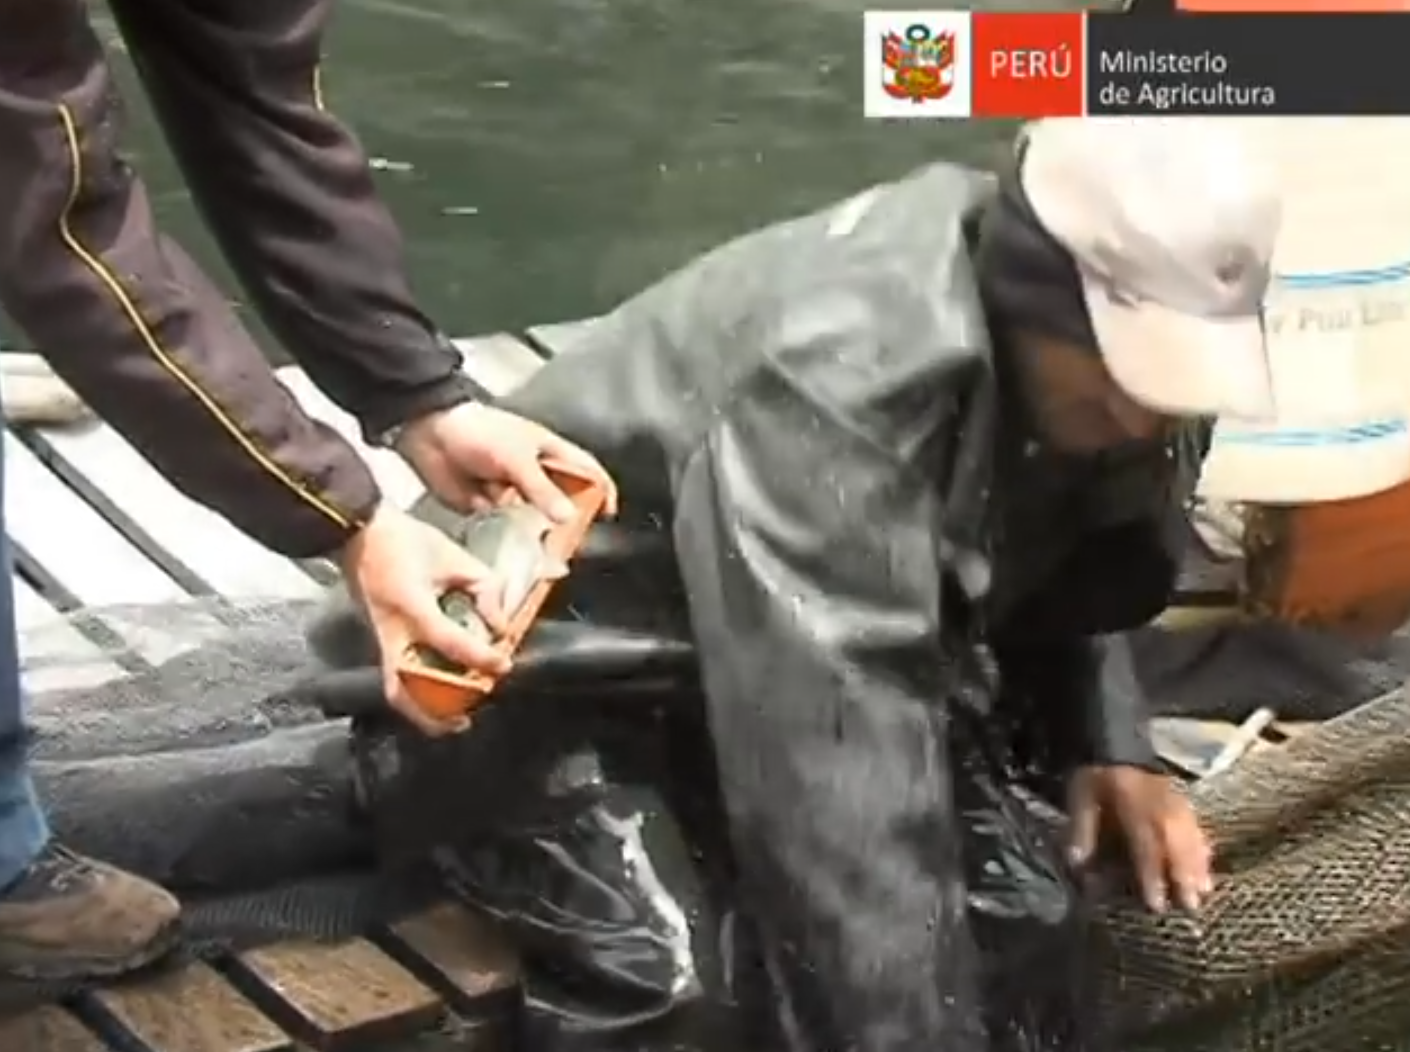
\includegraphics[width=0.65\textwidth]{chapter1/clasificacion y medicion manual de truchas.png}
		\caption{Clasificación y medición manual de truchas.}
		Fuente: MINAGRI\footnote{Ministerio de Agricultura y Riego del Perú.}.
		\label{fig:clasificacion y medicion manual de truchas}
	\end{figure}
\end{savenotes}

Para la medición se usa una herramienta, como la mostrada en la Figura \ref{fig:herramienta de medicion manual para peces},creada \textbf{artesanalmente} que contiene un ictiómetro para medir al pez mientras se realiza una clasificación o verificar el tamaño del pez. 

\begin{figure}[H]
	\centering
	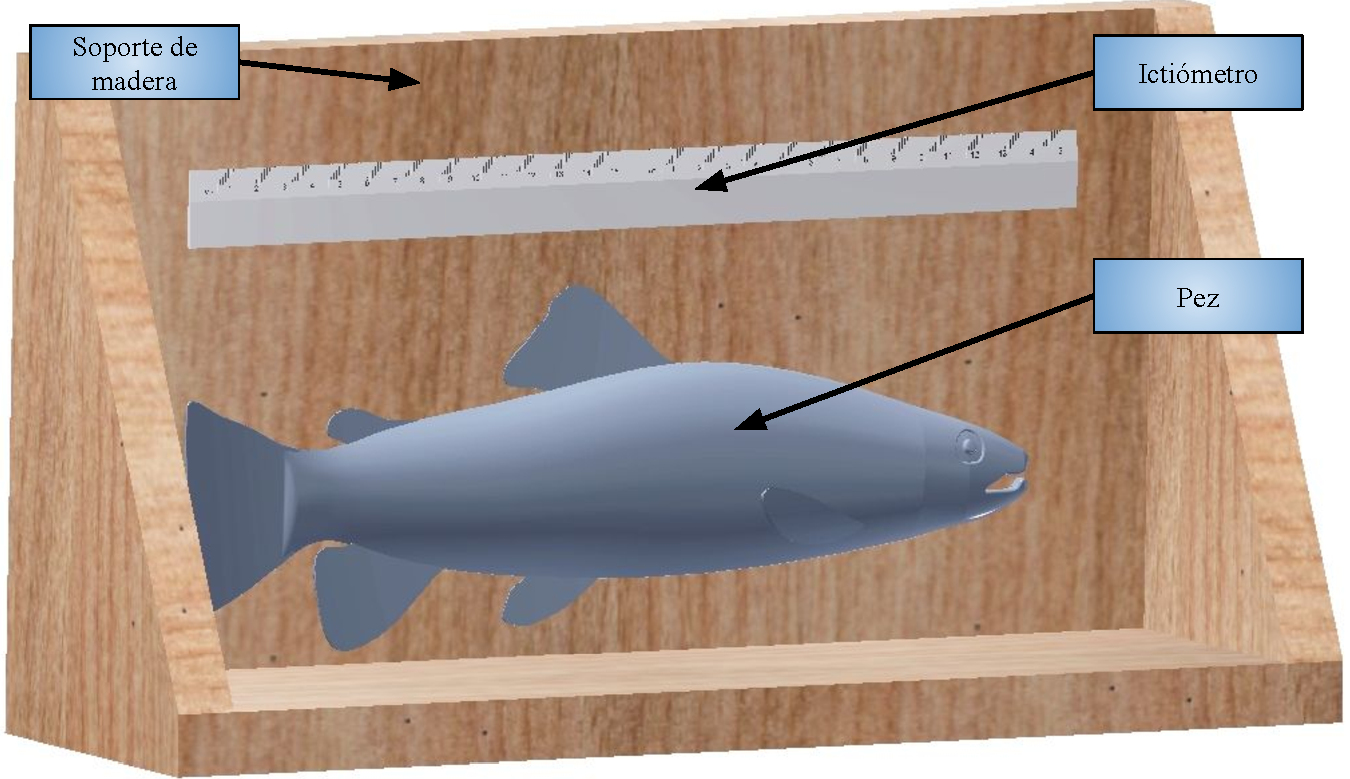
\includegraphics[width=0.75\textwidth]{chapter1/herramienta de medicion manual para peces.pdf}
	\caption{Herramienta de medición manual para peces.}
	Fuente: Elaboración propia.
	\label{fig:herramienta de medicion manual para peces}
\end{figure}

%% NUEVA SUB-SUB-SECCION X.X.X.X
\subsubsection{Clasificación mecánica}

La tesis que presentó el bachiller \textit{Angel Gabriel Vega De la Cruz} desarrolla un sistema mecánico que, asegura, permite seleccionar los peces de manera rápida y eficiente. El sistema mecánico consiste en un motorreductor, un sistema de alimentación compuesto por cuatro poleas y dos bandas transportadoras. La Figura \ref{fig:maquina seleccionadora de truchas agv} nos muestra la máquina, la cual puede clasificar tres rangos de  diferentes capacidades de selección (18 000, 7 200 y 3 600 peces/hora) a un precio estimado de S/ 19 264.27 en 2013. Otro factor importante es el peso de la máquina: 200 $ kg $.\citep[p.~2,105]{Vega2013}

\begin{figure}[H]
	\centering
	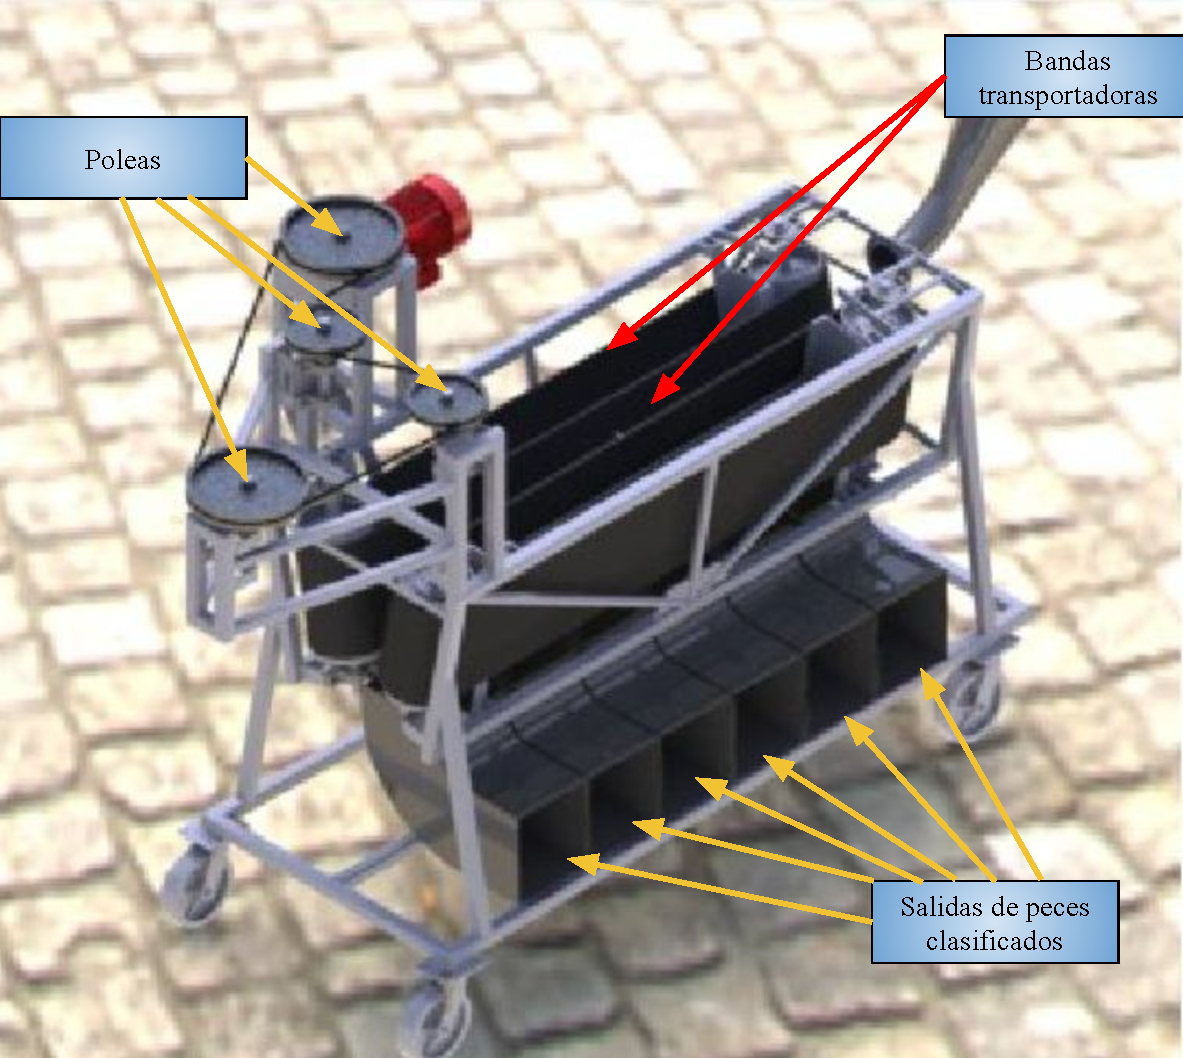
\includegraphics[width=0.65\textwidth]{chapter1/maquina seleccionadora de truchas agv.pdf}
	\caption{Máquina seleccionadora de truchas de A. G. V.}
	Fuente: Tesis “Diseño de una Máquina Seleccionadora de Truchas”.
	\label{fig:maquina seleccionadora de truchas agv}
\end{figure}

%% NUEVA SUB-SUB-SECCION X.X.X.X
\subsubsection{Clasificación mediante visión por computadora}

Este tipo de clasificación completamente automatizada permite un conteo de peces más rápido con respecto a otros métodos.\citep[p.~2-3]{Niu2018} Los avances en esta área son abundantes, en la Figura \ref{fig:medicion automatizada de especies y tallas de peces por vision artificial} se muestra uno de estos, una segmentación partiendo de la imagen de un pez.

\begin{figure}[H]
	\centering
	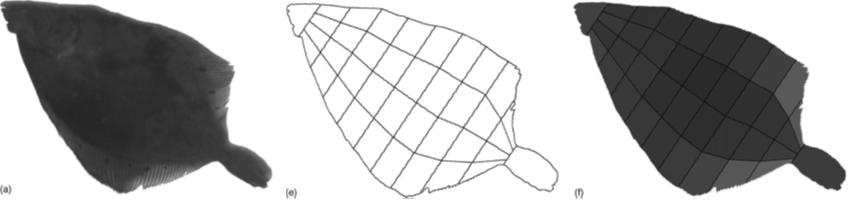
\includegraphics[width=1\textwidth]{chapter1/medicion automatizada de especies y tallas de peces por vision artificial.png}
	\caption{Medición automatizada de especies y tallas de peces por visión artificial.}
	(a,c,f) Imagen original, 100 puntos de borde y enmallado. \\
	Fuente: \citep[p.~4]{White2006}.
	\label{fig:medicion automatizada de especies y tallas de peces por vision artificial}
\end{figure}

En la Figura \ref{fig:medicion de peces dentro de estanques con camaras ortogonales y estereo} se muestra dos métodos para extraer la medida real de un pez para poder ser clasificado. El primero muestra un arreglo ortogonal de cámaras, en el caso de poder acceder en dos planos del estanque. El segundo muestra un arreglo que permite medir distancias entre puntos de interés mediante el uso de solo un plano del estanque.

\begin{figure}[H]
	\centering
	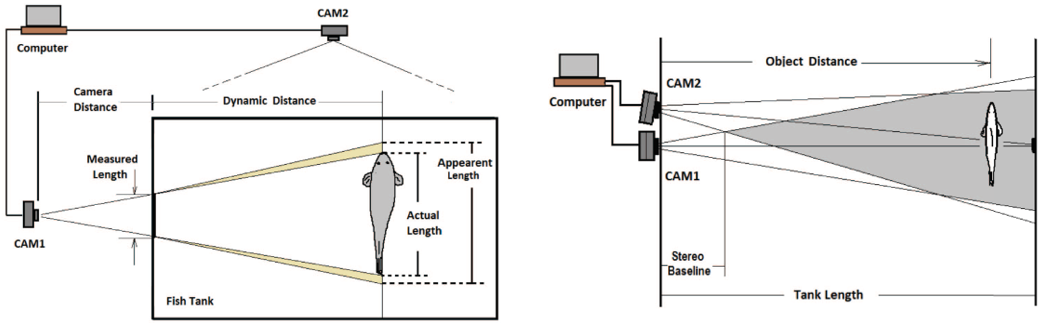
\includegraphics[width=1\textwidth]{chapter1/medicion de peces dentro de estanques con camaras ortogonales y estereo.png}
	\caption{Medición de  peces dentro de estanques con cámaras ortogonales y estéreo.}
	Fuente: \citep{Al-Jubouri2017}.
	\label{fig:medicion de peces dentro de estanques con camaras ortogonales y estereo}
\end{figure}


%En la Figura \ref{fig:medicion de peces dentro de estanques con camaras ortogonales} y Figura \ref{fig:medicion de peces dentro de estanques con camaras estereo} se muestra dos métodos para extraer la medida real de un pez para poder ser clasificado. El primero muestra un arreglo ortogonal de cámaras, en el caso de poder acceder en dos planos del estanque. El segundo muestra un arreglo que permite medir distancias entre puntos de interés mediante el uso de solo un plano del estanque.

%% NUEVA SUB-SUB-SECCION X.X.X.X
\subsubsection{Clasificación usando técnicas de inteligencia artificial}

Esta tecnología es robusta, es decir, funciona aceptablemente con ruido, cambios en condiciones ambientales, cambios en la adquisición de datos, entre otros cambios. La técnica se basa en redes neuronales\footnote{Las redes neuronales son usadas para modelar libremente la forma en que un cerebro biológico parametriza datos.}, con las que se logra una gran precisión para detectar y segmentar objetos en muchas diferentes condiciones (en este caso peces).\\

\begin{figure}[H]
	\centering
	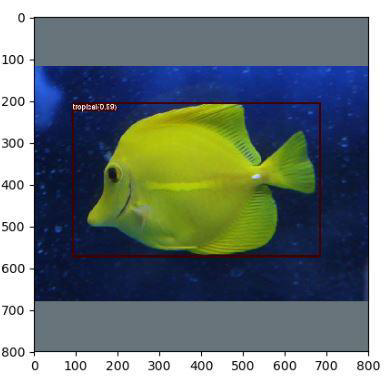
\includegraphics[width=0.5\textwidth]{chapter1/pez identificado por una red neuronal.png}
	\caption{Pez identificado por una red neuronal.}
	Fuente: \citep{Varalakshmi2019}.
	\label{fig:pez identificado por una red neuronal}
\end{figure}

%Este tipo de técnicas dependen de muchas variables y factores, en la Tabla \ref{tbl:comparacion de diferentes funciones de activacion} se muestra los principales, con los cuales se logra una mejor precisión de clasificación. \\

% Please add the following required packages to your document preamble:
% \usepackage[table,xcdraw]{xcolor}
% If you use beamer only pass "xcolor=table" option, i.e. \documentclass[xcolor=table]{beamer}
% Please add the following required packages to your document preamble:
% \usepackage[table,xcdraw]{xcolor}
% If you use beamer only pass "xcolor=table" option, i.e. \documentclass[xcolor=table]{beamer}

%\begin{table}[H]
%	\centering	
%	\caption{Comparación de diferentes funciones de activación.}
%	\label{tbl:comparacion de diferentes funciones de activacion}
%	\begin{tabular}{|c|c|c|c|c|c|c|}
%		\hline
%		\rowcolor[HTML]{A6A6A6} 
%		{\color[HTML]{000000} \textbf{N°}} & {\color[HTML]{000000} \textbf{\begin{tabular}[c]{@{}c@{}}Capa\\ convolucional\end{tabular}}} & {\color[HTML]{000000} \textbf{\begin{tabular}[c]{@{}c@{}}Capa\\ reductora\end{tabular}}} & {\color[HTML]{000000} \textbf{\begin{tabular}[c]{@{}c@{}}Capa \\ completamente\\ conectada\end{tabular}}} & {\color[HTML]{000000} \textbf{Epoch}} & {\color[HTML]{000000} \textbf{Precisión}} & {\color[HTML]{000000} \textbf{\begin{tabular}[c]{@{}c@{}}Funciones\\ de\\ activación\end{tabular}}} \\ \hline
%		{\color[HTML]{000000} 1} & {\color[HTML]{000000} 2} & {\color[HTML]{000000} 2} & {\color[HTML]{000000} 2} & {\color[HTML]{000000} 50} & {\color[HTML]{000000} 95\%} & {\color[HTML]{000000} ReLu,   Sigmoid} \\ \hline
%		{\color[HTML]{000000} 2} & {\color[HTML]{000000} 2} & {\color[HTML]{000000} 2} & {\color[HTML]{000000} 2} & {\color[HTML]{000000} 50} & {\color[HTML]{000000} 50\%} & {\color[HTML]{000000} ReLu,   Softmax} \\ \hline
%		{\color[HTML]{000000} 3} & {\color[HTML]{000000} 4} & {\color[HTML]{000000} 4} & {\color[HTML]{000000} 4} & {\color[HTML]{000000} 50} & {\color[HTML]{000000} 48\%} & {\color[HTML]{000000} ReLu,   Sigmoid} \\ \hline
%	\end{tabular}
%	\\ Fuente: \citep{Varalakshmi2019}.
%\end{table}

%% NUEVA SUB-SUB-SECCION X.X.X.X
\subsubsection{Comparación}

La Tabla \ref{tbl:comparacion entre metodos de clasificacion} desarrolla una comparación tanto cuantitativa como cualitativa de los métodos de clasificación de peces. \textbf{La cantidad de peces por hora} se refiere a la máxima cantidad que se puede clasificar en una hora según el método. \textbf{El mantenimiento} es la frecuencia en la cual la máquina pasa una inspección para verificar su correcto funcionamiento. El \textbf{costo de implementación} se refiere al costo de diseñar e implementar el método. El \textbf{costo de funcionamiento} se refiere al consumo energético en general del empleo del método. La \textbf{precisión} se refiere a la cantidad de peces bien clasificados en el proceso. La calificación “bajo, medio, alto” son juicios del autor, basándose en su experiencia.

% Please add the following required packages to your document preamble:
% \usepackage[table,xcdraw]{xcolor}
% If you use beamer only pass "xcolor=table" option, i.e. \documentclass[xcolor=table]{beamer}
\begin{table}[H]
	\centering
	\caption{Comparación entre los métodos de clasificación.}
	\label{tbl:comparacion entre metodos de clasificacion}
	\begin{tabular}{|l|c|c|c|c|}
		\hline
		\rowcolor[HTML]{A6A6A6} 
		\multicolumn{1}{|c|}{\cellcolor[HTML]{A6A6A6}{\color[HTML]{000000} \textbf{Criterio\textbackslash{}Método}}} & {\color[HTML]{000000} \textbf{Manual}} & {\color[HTML]{000000} \textbf{Mecánico}} & {\color[HTML]{000000} \textbf{\begin{tabular}[c]{@{}c@{}}Visión por\\  computadora\end{tabular}}} & {\color[HTML]{000000} \textbf{\begin{tabular}[c]{@{}c@{}}Inteligencia \\ Artificial\end{tabular}}} \\ \hline
		{\color[HTML]{000000} \begin{tabular}[c]{@{}l@{}}Cantidad de peces \\ por hora\end{tabular}} & {\color[HTML]{000000} \begin{tabular}[c]{@{}c@{}}120\\ (por operario)\end{tabular}} & {\color[HTML]{000000} 18000} & {\color[HTML]{000000} \begin{tabular}[c]{@{}c@{}}Según capacidad \\ de cómputo\end{tabular}} & {\color[HTML]{000000} \begin{tabular}[c]{@{}c@{}}Según capacidad\\ de cómputo\end{tabular}} \\ \hline
		{\color[HTML]{000000} Mantenimiento} & {\color[HTML]{000000} -} & {\color[HTML]{000000} Semestral} & {\color[HTML]{000000} Anual} & {\color[HTML]{000000} Anual} \\ \hline
		{\color[HTML]{000000} \begin{tabular}[c]{@{}l@{}}Costo de \\ implementación\end{tabular}} & {\color[HTML]{000000} Bajo} & {\color[HTML]{000000} Medio} & {\color[HTML]{000000} Medio} & {\color[HTML]{000000} Medio} \\ \hline
		{\color[HTML]{000000} \begin{tabular}[c]{@{}l@{}}Costo de \\ funcionamiento\end{tabular}} & {\color[HTML]{000000} Bajo} & {\color[HTML]{000000} Bajo} & {\color[HTML]{000000} Medio} & {\color[HTML]{000000} Alto} \\ \hline
		{\color[HTML]{000000} Precisión} & {\color[HTML]{000000} Media} & {\color[HTML]{000000} Alta} & {\color[HTML]{000000} Alta} & {\color[HTML]{000000} Muy alta} \\ \hline
	\end{tabular}
	\\ Fuente: Elaboración Propia.
\end{table}

%% NUEVO SUBSECCION X.X.X
\subsection{Sistema de conteo de peces}

El proceso se realiza como método para calcular la \textbf{biomasa}\footnote{La masa total de peces en un volumen determinado, se usa para determinar la cantidad de alimentación.}, verificar la \textbf{mortandad} y con propósitos de venta. Se realiza un conteo del pez directa o indirectamente. 

%% NUEVA SUB-SUB-SECCION X.X.X.X
\subsubsection{Conteo manual}

Debido a que realizar de forma separada y manual los procesos de clasificación, conteo o curado\footnote{Proceso de aplicar sal marina a los peces con la finalidad de sanar de enfermedades como \textit{saprolegniosis} o \textit{exoftalmia}.}  de truchas requeriría de excesivo tiempo y operarios, se suele realizar los tres procesos de manera como si de un solo proceso se tratase como se muestra en la Figura \ref{fig:clasificacion conteo curado y calculo de biomasa en la laguna de canrash}. El proceso resultante contempla los tres subprocesos de manera secuencial: extracción de la trucha de los estanques o jaulas flotantes, curado, clasificación, conteo y cálculo de biomasa en un determinado recipiente.\\

\begin{figure}[H]
	\centering
	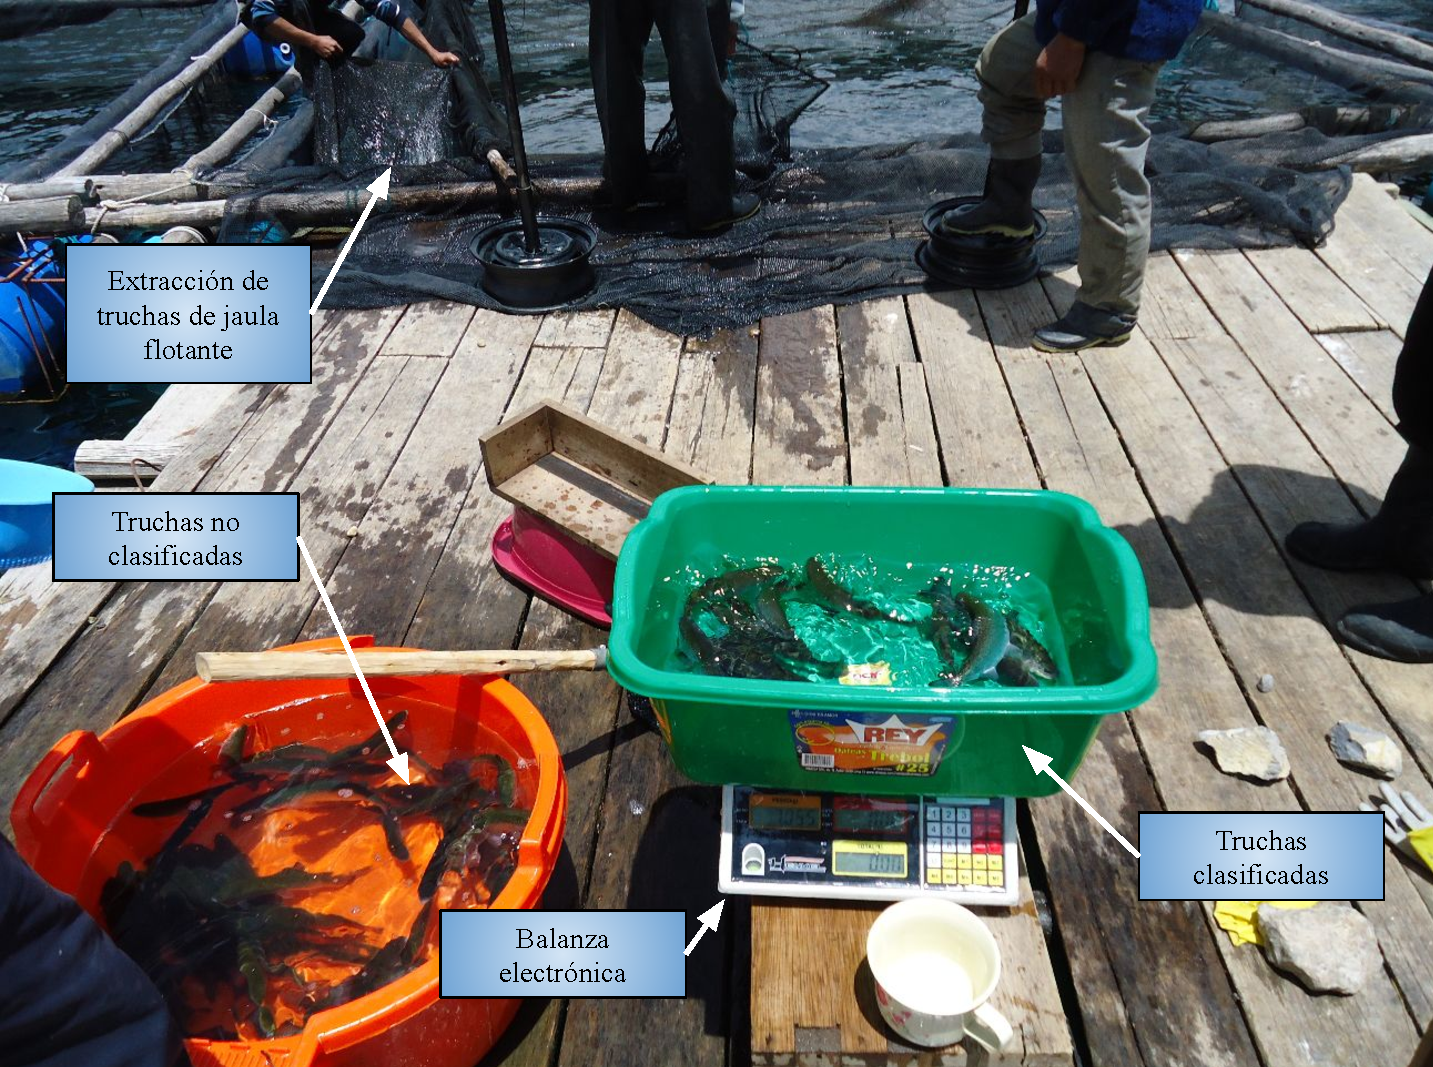
\includegraphics[width=1\textwidth]{chapter1/clasificacion conteo curado y calculo de biomasa en la laguna de canrash.pdf}
	\caption{Clasificación, conteo, curado y cálculo de biomasa en la laguna de Canrash, Ancash, Perú.}
	Fuente: Elaboración propia.
	\label{fig:clasificacion conteo curado y calculo de biomasa en la laguna de canrash}
\end{figure}

%% NUEVA SUB-SUB-SECCION X.X.X.X
\subsubsection{Conteo por sensores}

Este tipo de conteo se basa en el uso de sensores en general (láseres, ultrasonidos, presencia, capacitivos, entre otros).  El contador que se muestra en la Figura \ref{fig:contador peces basado en luz infrarroja faivre} realiza un conteo mediante el uso de láseres infrarrojos que forman una \textit{cortina}\footnote{Llamada también barrera.}. El pez en tránsito impide que el láser llegue al lado opuesto en el cual se recibe la luz en un sensor receptivo, generando así un control lógico sobre la presencia del pez. Con la finalidad de evitar mal conteo por superposición de los peces se suele tener un sistema que canaliza un pez a la vez que pase por el sistema contador.

\begin{figure}[H]
	\centering
	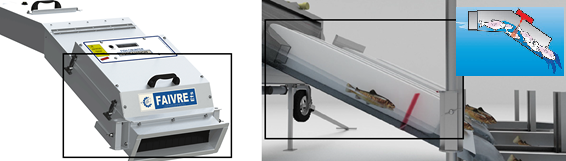
\includegraphics[width=1\textwidth]{chapter1/contador peces basado en luz infrarroja faivre.png}
	\caption{Contador de peces basado en luz infrarroja.}
	Fuente: \citep{FAIVRE2013}.
	\label{fig:contador peces basado en luz infrarroja faivre}
\end{figure}

%% NUEVA SUB-SUB-SECCION X.X.X.X
\subsubsection{Conteo mediante visión por computadora}

El proceso de conteo mediante visión por computadora se realiza a partir de una imagen capturada desde un plano específico como se muestra en la  Figura \ref{fig:planos comunes de posicionamiento para camaras de inspeccion}. Dicha imagen se procesa para poder realizar una segmentación adecuada de la trucha y así poder contabilizarlas. El número de cámaras y las posiciones varían dependiendo de qué se busca.

\begin{figure}[H]
	\centering
	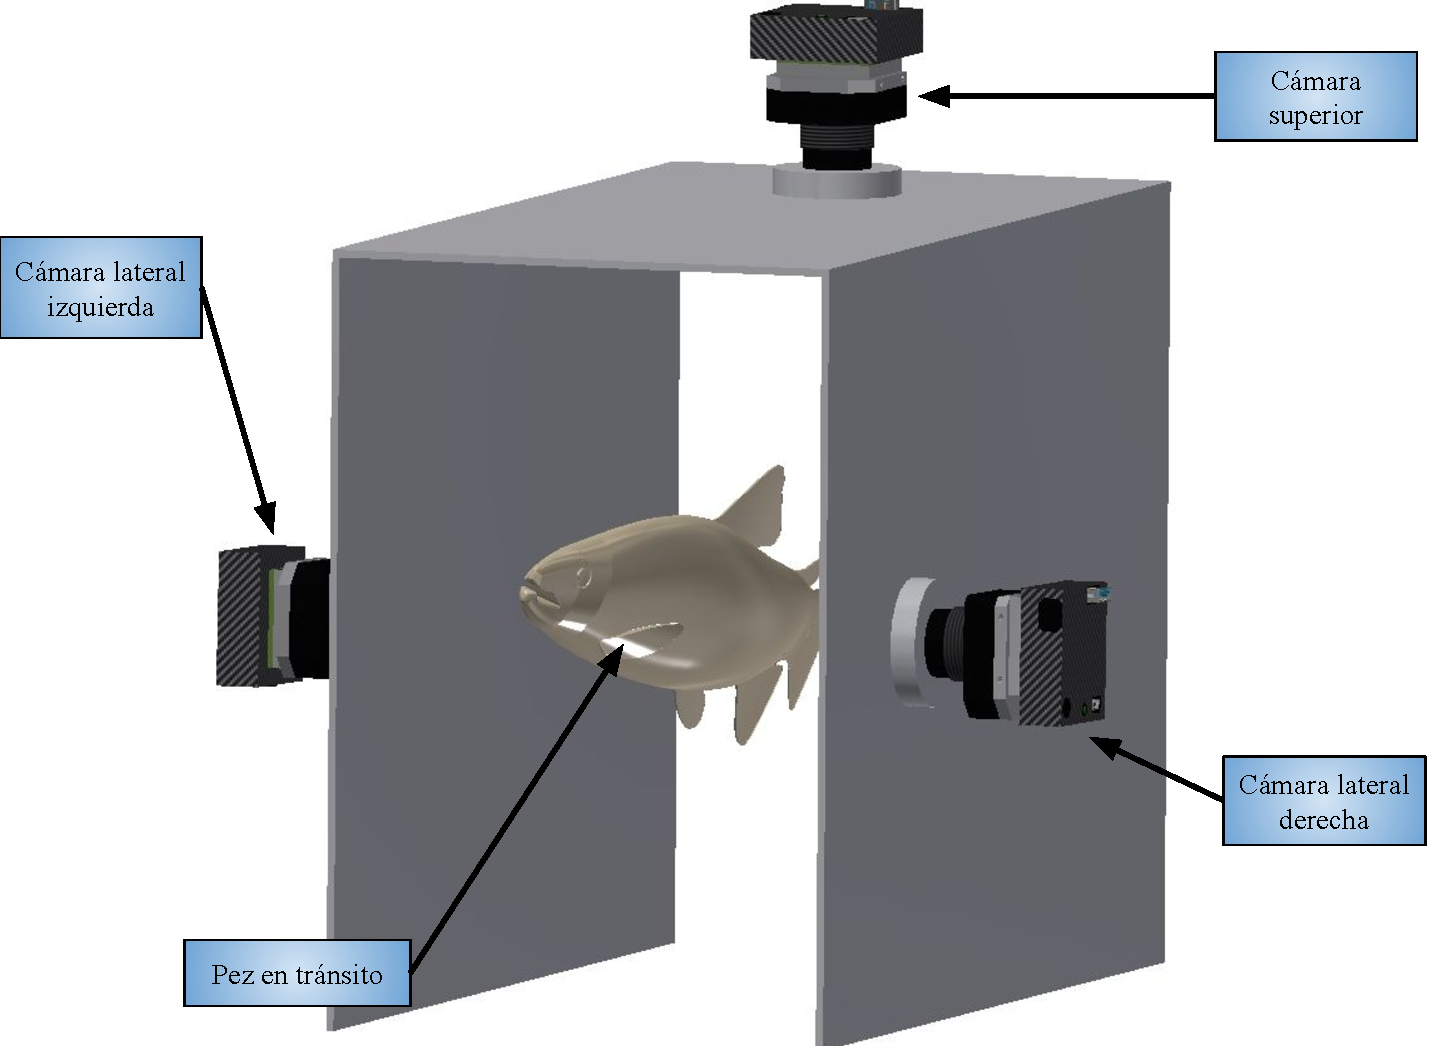
\includegraphics[width=0.8\textwidth]{chapter1/planos comunes de posicionamiento para camaras de inspeccion.pdf}
	\caption{Planos comunes de posicionamiento para cámaras de inspección.}
	Fuente: Elaboración propia.
	\label{fig:planos comunes de posicionamiento para camaras de inspeccion}
\end{figure}

%% NUEVA SUB-SUB-SECCION X.X.X.X
\subsubsection{Conteo mixto}

El conteo mixto\footnote{Método que emplea sensores y visión por computadora.} se realiza usando imágenes, electrónica y software para aumentar la precisión del conteo. El fabricante afirma tener una alta precisión, sistema fácil de usar, sistema fácil de movilizar y en un tiempo corto. \citep{AquaScan2015}

\begin{figure}[H]
	\centering
	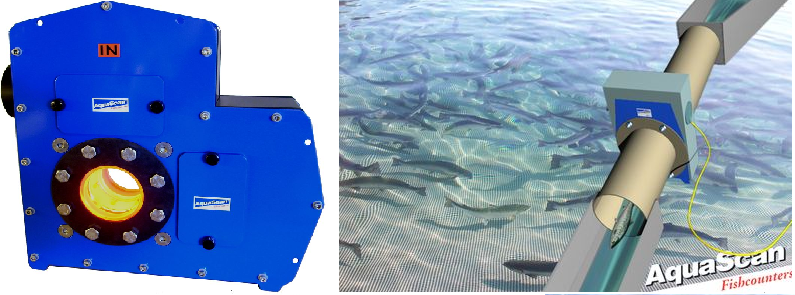
\includegraphics[width=1\textwidth]{chapter1/contador de peces mediante escaneres.png}
	\caption{Contador de peces mediante escáneres.}
	Fuente: Elaboración propia.
	\label{fig:contador de peces mediante escaneres}
\end{figure}

%% NUEVA SUB-SUB-SECCION X.X.X.X
\subsubsection{Comparación}

En la Tabla \ref{tbl:comparacion entre metodos de conteo de peces} desarrolla una comparación tanto cuantitativa como cualitativa de los métodos de conteo de peces. \textbf{La cantidad de peces por hora} se refiere a la cantidad de peces que puede contar en una hora. El \textbf{mantenimiento} se refiere a la frecuencia con la cual se inspecciona el funcionamiento correcto del método. El \textbf{costo de implementación} y \textbf{de funcionamiento} se refieren a los costos de diseño, implementación y de marcha. La \textbf{precisión} se refiere a la cantidad de peces correctamente contados en comparación con los que no fueron contados. La calificación “\textit{bajo, medio, alto}” son juicios del autor, basándose en su experiencia.


% Please add the following required packages to your document preamble:
% \usepackage[table,xcdraw]{xcolor}
% If you use beamer only pass "xcolor=table" option, i.e. \documentclass[xcolor=table]{beamer}
\begin{table}[H]
	
	\centering
	\caption{Comparación entre los métodos de conteo de peces.}
	\label{tbl:comparacion entre metodos de conteo de peces}
	\begin{tabular}{|
			>{\columncolor[HTML]{D9D9D9}}l |c|c|c|c|}
		\hline
		\cellcolor[HTML]{A6A6A6}{\color[HTML]{000000} \textbf{Criterio\textbackslash{}Método}} &
		\cellcolor[HTML]{A6A6A6}{\color[HTML]{000000} \textbf{Manual}} &
		\cellcolor[HTML]{A6A6A6}{\color[HTML]{000000} \textbf{Sensores}} &
		\cellcolor[HTML]{A6A6A6}{\color[HTML]{000000} \textbf{\begin{tabular}[c]{@{}c@{}}Visión por \\ computadora\end{tabular}}} &
		\cellcolor[HTML]{A6A6A6}{\color[HTML]{000000} \textbf{Mixto}} \\ \hline
		{\color[HTML]{000000} \begin{tabular}[c]{@{}l@{}}Cantidad de peces\\ por hora\end{tabular}} &
		{\color[HTML]{000000} \begin{tabular}[c]{@{}c@{}}120\\ (por operario)\end{tabular}} &
		{\color[HTML]{000000} 95000} &
		{\color[HTML]{000000} \begin{tabular}[c]{@{}c@{}}Según capacidad \\ de cómputo\end{tabular}} &
		{\color[HTML]{000000} \begin{tabular}[c]{@{}c@{}}Según capacidad \\ de cómputo\end{tabular}} \\ \hline
		{\color[HTML]{000000} Mantenimiento} &
		{\color[HTML]{000000} -} &
		{\color[HTML]{000000} Semestral} &
		{\color[HTML]{000000} Anual} &
		{\color[HTML]{000000} Anual} \\ \hline
		{\color[HTML]{000000} \begin{tabular}[c]{@{}l@{}}Costo de \\ implementación\end{tabular}} &
		{\color[HTML]{000000} Bajo} &
		{\color[HTML]{000000} Bajo} &
		{\color[HTML]{000000} Medio} &
		{\color[HTML]{000000} Medio} \\ \hline
		{\color[HTML]{000000} \begin{tabular}[c]{@{}l@{}}Costo de\\ funcionamiento\end{tabular}} &
		{\color[HTML]{000000} Bajo} &
		{\color[HTML]{000000} Bajo} &
		{\color[HTML]{000000} Alto} &
		{\color[HTML]{000000} Alto} \\ \hline
		{\color[HTML]{000000} Precisión} &
		{\color[HTML]{000000} Media} &
		{\color[HTML]{000000} Alta} &
		{\color[HTML]{000000} Alta} &
		{\color[HTML]{000000} Muy alta} \\ \hline
	\end{tabular}
\\ Fuente: Elaboración propia.
\end{table}

%% NUEVO SUBSECCION X.X.X
\subsection{Extracción de características de peces}

“La evaluación del comportamiento o fisiología de los peces cultivados siempre ha sido difícil debido al tiempo de muestreo, la-s diferencias entre las condiciones experimentales y el sesgo metodológico inherente. Sin embargo, los recientes avances en la tecnología de visión artificial\footnote{Elsevier afirma que la tecnología de visión por computadora se considera existente desde 1973 hasta la fecha.} han abierto posibilidades para observar mejor el comportamiento de los peces. Tal tecnología permite herramientas de inspección no destructivas, rápidas, económicas, consistentes y objetivas, mientras que proporcionando técnicas de evaluación basadas en el análisis y procesamiento de imágenes en una amplia variedad de aplicaciones”.\citep[p.~1]{Niu2018}

%% NUEVA SUB-SUB-SECCION X.X.X.X
\subsubsection{Extracción mediante inspección visual}

En el subíndice \textbf{\ref{ssec:sistema de clasificacion de peces}} se explica sobre el uso de herramientas para poder medir al pez. Mientras se toma la medida un profesional o técnico acuícola realiza una inspección visual para detectar enfermedades víricas, bacterianas o fúngicas visibles.

%% NUEVA SUB-SUB-SECCION X.X.X.X
\subsubsection{Extracción de características mediante visión por computadora}

La empresa acuícola noruega \textit{Cermaq Group AS} está planeando la implementación de un sistema de reconocimiento facial como parte de un proyecto de última tecnología llamada iFarm.\citep{Daley2018} Este tipo de técnicas se recomienda para medianas y grandes empresas debido al alto costo de implementación y mantenimiento. Las principales ventajas, a diferencia de métodos tradicionales, son la personalización y seguimiento de cada pez analizado, es decir, se puede tener un reporte de vida de cada trucha. Esta innovación brinda una precisión muy alta ya que suele ser apoyada por algoritmos de inteligencia artificial que brindan robustez al sistema. Gracias al análisis personalizado se puede identificar los principales problemas que aquejan a los peces, a diferencia del análisis general que se realiza comúnmente. Según la empresa, este método disminuye la mortandad de 50\% a 25\% en todo el proceso de cultivo. En la Figura \ref{fig:extraccion de caracteristicas mediante vision por computadora} se ejemplifica el reporte.

\begin{figure}[H]
	\centering
	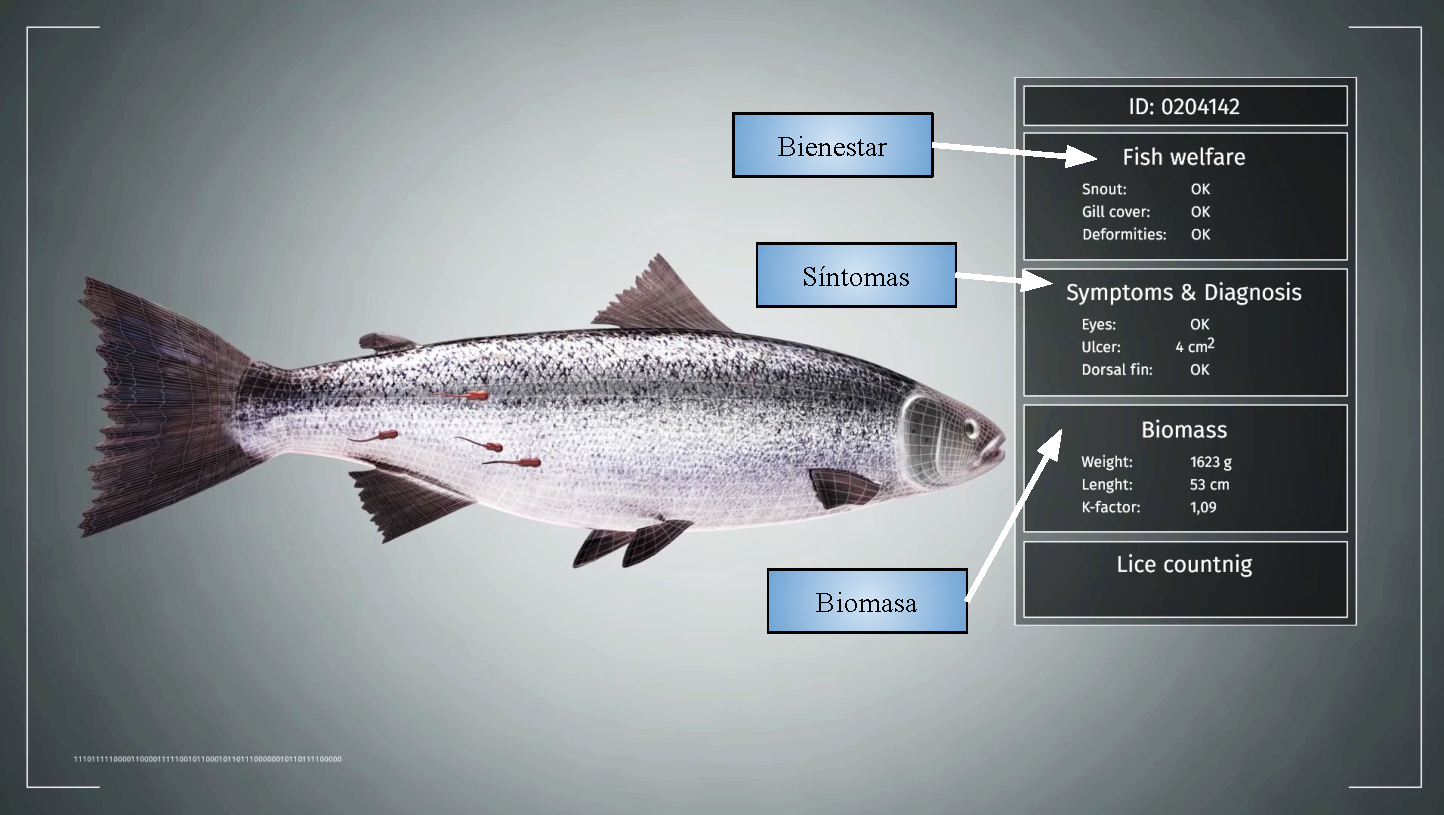
\includegraphics[width=1\textwidth]{chapter1/extraccion de caracteristicas mediante vision por computadora.pdf}
	\caption{Extracción de características mediante visión por computadora.}
	Fuente: \citep{Biosort2016}
	\label{fig:extraccion de caracteristicas mediante vision por computadora}
\end{figure}

Hao M. diseño un sistema de visión artificial que puede medir con precisión la longitud de los peces, tiene dos tipos de funcionamiento del sistema. El primer tipo solo usa una imagen y posee una referencia para poder estimar la longitud del pez a través de la transformación de Hough (Figura \ref{fig:usando relacion entre a y b para calcular longitud del pez}). El segundo tipo usa más imágenes para realizar un modelo 3d, la investigación indica que el sistema funciona con precisión. \citep[p.~4-5]{Niu2018}

\begin{figure}[H]
	\centering
	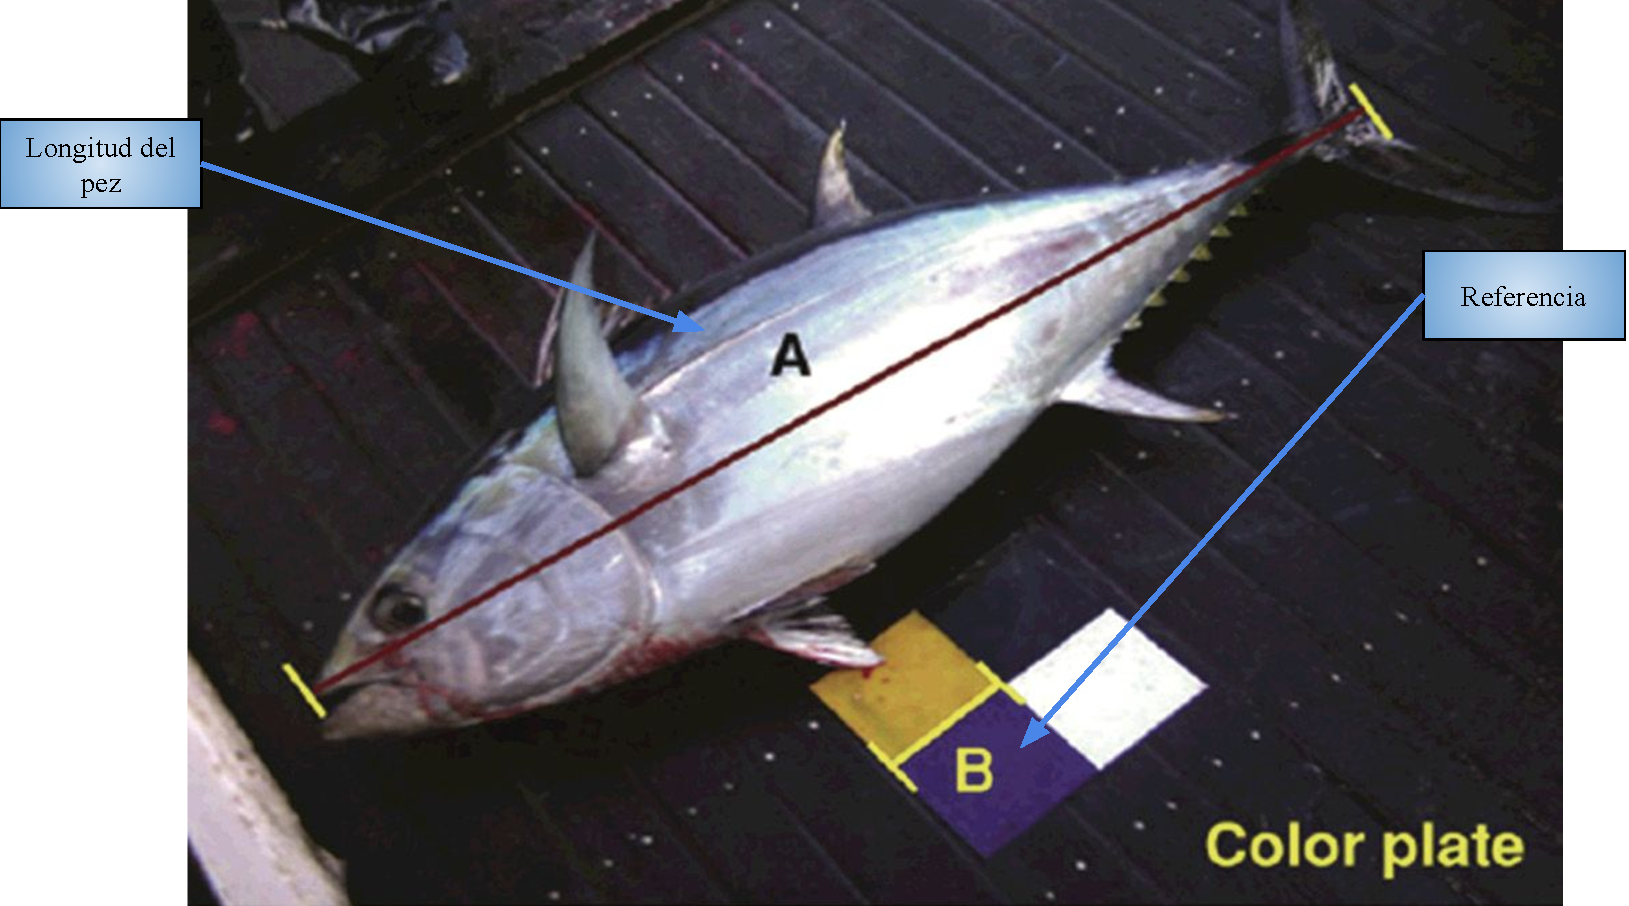
\includegraphics[width=0.85\textwidth]{chapter1/usando relacion entre a y b para calcular longitud del pez.pdf}
	\caption{Usando la relación  entre A y B para calcular la longitud del pez.}
	Fuente: \citep{Hao2016}
	\label{fig:usando relacion entre a y b para calcular longitud del pez}
\end{figure}

%% NUEVO SUBSECCION X.X.X
\subsection{Sistema de traslado de peces}

El proceso de llevar un pez de un estanque o jaula flotante a un lugar específico se denomina traslado. Dicho traslado es necesario al momento de clasificar, contar y procesar en general al pez. Durante el cultivo de trucha esta práctica se repite con frecuencia, y en caso no fuera empleada de manera correcta el pez puede morir.

%% NUEVA SUB-SUB-SECCION X.X.X.X
\subsubsection{Traslado manual}

Los operarios usan redes en un cabezal metálico en forma circular apoyados por un palo metálico o de madera para trasladar a las truchas\footnote{También son llamadas sacaderas telescópicas.}.

\begin{figure}[H]
	\centering
	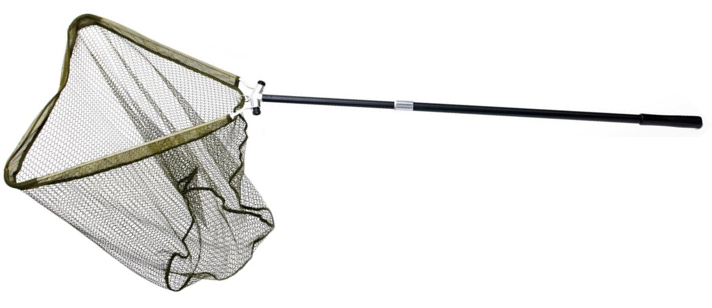
\includegraphics[width=1\textwidth]{chapter1/sacadera telescipica de malla fina para peces.png}
	\caption{Usando la relación  entre A y B para calcular la longitud del pez.}
	Fuente: Seomusen vía Amazon.
	\label{fig:sacadera telescipica de malla fina para peces}
\end{figure}

%% NUEVA SUB-SUB-SECCION X.X.X.X
\subsubsection{Traslado automático}

En la Figura \ref{fig:recepcion automatica por bombeo de peces mediante tuberia} se muestra cómo se recepciona los peces en tránsito que están dentro de una tubería que son impulsadas por una corriente de agua, generada posiblemente por una bomba para peces\footnote{También llamada bomba "\textit{pin pin}", realiza una función similar a una bomba centrífuga, pero con peces en lugar de solo agua.}.

\begin{figure}[H]
	\centering
	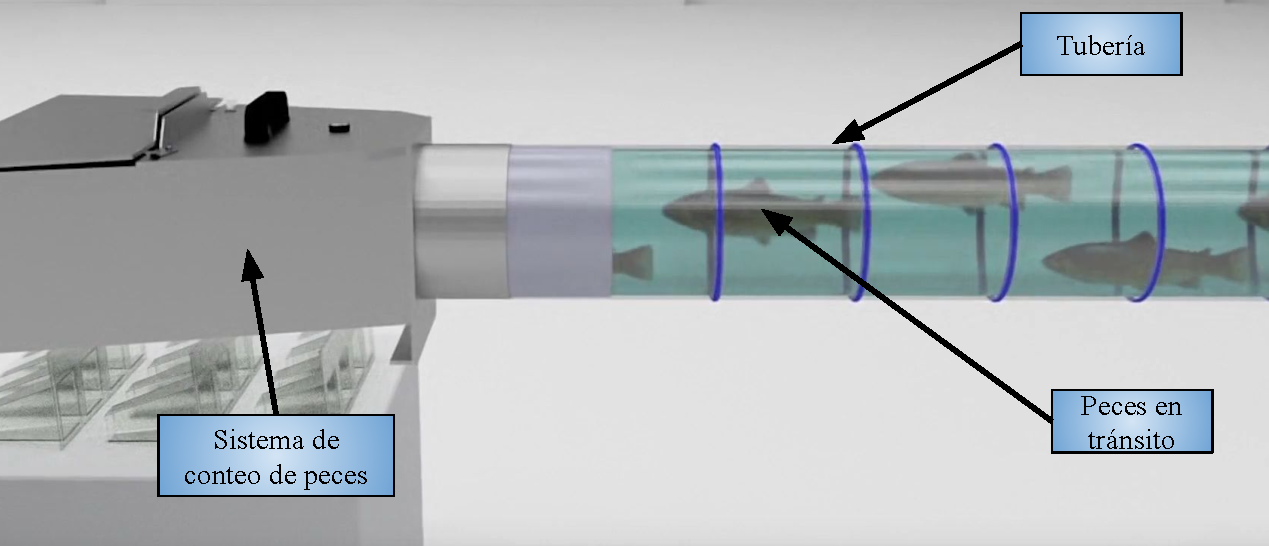
\includegraphics[width=1\textwidth]{chapter1/recepcion automatica por bombeo de peces mediante tuberia.pdf}
	\caption{Recepción automática por bombeo de peces mediante tubería.}
	Fuente: Videos recopilados de FAIVRE
	\label{fig:recepcion automatica por bombeo de peces mediante tuberia}
\end{figure}

%% NUEVA SUB-SUB-SECCION X.X.X.X
\subsubsection{Comparación}

En la Tabla \ref{tbl:comparacion entre los metodos de traslado de peces} desarrolla una comparación tanto cuantitativa como cualitativa de los métodos de conteo de peces. La \textbf{cantidad de peces por hora} se refiere a la cantidad de peces que puede transportar en una hora. El \textbf{mantenimiento} se refiere a la frecuencia con la cual se inspecciona el funcionamiento correcto del método. El \textbf{costo de implementación} y de \textbf{funcionamiento} se refieren a los costos de diseño, implementación y de marcha. La precisión se refiere a la cantidad de peces trasladados que no mueren. La calificación “\textit{bajo, medio, alto}” son juicios del autor, basándose en su experiencia.

% Please add the following required packages to your document preamble:
% \usepackage[table,xcdraw]{xcolor}
% If you use beamer only pass "xcolor=table" option, i.e. \documentclass[xcolor=table]{beamer}
\begin{table}[H]	
	\centering
	\caption{Comparación entre los métodos de traslado de peces.}
	\label{tbl:comparacion entre los metodos de traslado de peces}
	\begin{tabular}{|
			>{\columncolor[HTML]{D9D9D9}}l |c|c|}
		\hline
		\multicolumn{1}{|c|}{\cellcolor[HTML]{A6A6A6}{\color[HTML]{000000} \textbf{Criterio\textbackslash{}Método}}} &
		\cellcolor[HTML]{A6A6A6}{\color[HTML]{000000} \textbf{Manual}} &
		\cellcolor[HTML]{A6A6A6}{\color[HTML]{000000} \textbf{Automático}} \\ \hline
		{\color[HTML]{000000} Cantidad de peces por hora} &
		{\color[HTML]{000000} \begin{tabular}[c]{@{}c@{}}360 aproximadamente\\ (por operario)\end{tabular}} &
		{\color[HTML]{000000} 20000} \\ \hline
		{\color[HTML]{000000} Mantenimiento}           & {\color[HTML]{000000} -}    & {\color[HTML]{000000} Semestral} \\ \hline
		{\color[HTML]{000000} Costo de implementación} & {\color[HTML]{000000} Bajo} & {\color[HTML]{000000} Alto}      \\ \hline
		{\color[HTML]{000000} Costo de funcionamiento} & {\color[HTML]{000000} Bajo} & {\color[HTML]{000000} Alto}      \\ \hline
		{\color[HTML]{000000} Precisión}               & {\color[HTML]{000000} Bajo} & {\color[HTML]{000000} Medio}     \\ \hline
	\end{tabular}
	\\ Fuente: Elaboración propia.
\end{table}

%% NUEVO SUBSECCION X.X.X
\subsection{Productos comerciales y patentes}
\label{ssec:productos comerciales y patentes}

En el mercado internacional se distribuyen máquinas que realizan la clasificación, conteo o ambos de manera semiautomática y completamente automática. 

%% NUEVA SUB-SUB-SECCION X.X.X.X
\subsubsection{Dispositivo de clasificación de peces y método de clasificación de peces \textit{(Patente JP5563164B2)}}

El control de la clasificación de los peces se realiza por límites de peso, es decir, se asigna dos límites en gramos y este dispositivo logra separar la entrada de peces en tres rangos. La máquina trabaja con peces vivos y permite, según los inventores, una clasificación rápida y precisa de un modo eficiente. La recepción de peces puede darse solo para un pez vivo a la vez. El compartimiento de clasificación mide 0.5 metros, llamado compartimento de pesaje. El ingreso de datos mediante una unidad de control que posee una interfaz de usuario y un dispositivo de memoria electrónica para ingresar y recepcionar datos. La invención, según los desarrolladores, es observar la diferencia de crecimiento comparando con anteriores clasificaciones para distribuirlos mejor en futuros estanques y controlar de una mejor manera la alimentación.\citep{2010}

\begin{figure}[H]
	\centering
	\rot{\rot{\rot{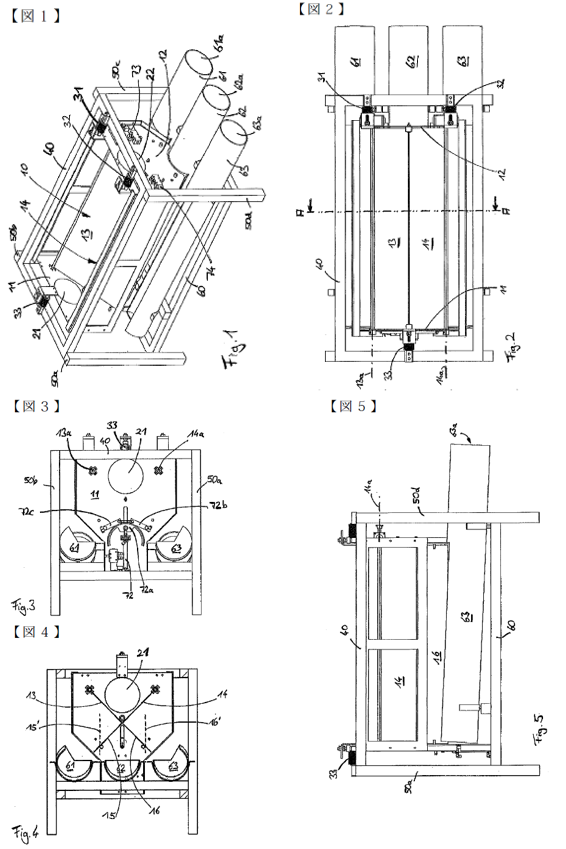
\includegraphics[width=0.70\textwidth]{chapter1/clasificadora automatica de peces de origen japones.png}}}}
	\caption{Clasificadora automática de peces de origen japonés.}
	Fuente: Patente JP5563164B2.
	\label{fig:clasificadora automatica de peces de origen japones}
\end{figure}

%% NUEVA SUB-SUB-SECCION X.X.X.X
\subsubsection{Clasificador completamente automático de pescado \textit{(Patente CN205180233U)}}

Este clasificador completamente automático incluye tres máquinas, la primera máquina elevadora, la segunda máquina elevadora y la tercera la niveladora. La salida de la primera máquina se encuentra en la parte superior de la entrada de la segunda máquina, la salida de la segunda máquina se encuentra en la parte superior de la entrada de la niveladora, conectado de forma fija con la bomba de agua en la segunda máquina de elevación. La ducha se fija en el marco de la primera salida de la máquina de elevación. Esto rectifica y mejora perfectamente al clasificador de peces debido a la rotación del cilindro de surtido.\citep{Fang2015} El fabricante usa tambores de rotación, configuraciones de elevación de peces para enfriar por pulverizado al pescado, reducir la viscosidad con el objetivo de evitar lesiones por uso y desgaste. Además, usa rodillos giratorios para evitar la mala clasificación de los pescados. No se especifica cantidades o porcentaje de error del uso.

\begin{figure}[H]
	\centering
	\rot{\rot{\rot{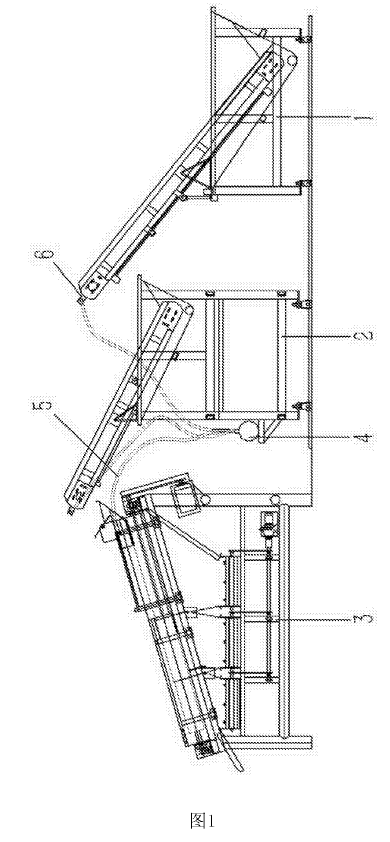
\includegraphics[width=0.45\textwidth]{chapter1/clasificadora automatica de peces de origen chino.png}}}}
	\caption{Clasificadora automática de peces de origen chino.}
	Fuente: Patente CN205180233U.
	\label{fig:clasificadora automatica de peces de origen chino}
\end{figure}

%% NUEVA SUB-SUB-SECCION X.X.X.X
\subsubsection{Clasificador y contador automático de peces \textit{(Patente CN203884438U)}}

Esta máquina comprende una máquina clasificadora automática y al menos una máquina contadora automática. La máquina de clasificación comprende un marco, las tuberías de salida de peces, cada máquina de conteo automático comprende un tanque de peces de conteo, un tubo de entrada de peces está dispuesto en un extremo de cada tanque de peces de conteo y cada tubo de cada salida de peces se comunica con la tubería de entrada de pescado correspondiente. El clasificador automático de peces tiene las ventajas de que los tamaños y las cantidades de peces se pueden distinguir con ayuda de las máquinas, por lo tanto, el tiempo de trabajo se puede reducir, la eficiencia de trabajo se puede mejorar en gran medida, se puede garantizar la precisión de los daos y se puede evitar lesiones y aumentar la tasa de supervivencia de los peces al pasar por este proceso.\citep{Jingwen2014} El inventor \textbf{no precisa} materiales de fabricación, cuantificación de la cantidad máxima de producción, porcentajes de error u otros puntos específicos.

\begin{figure}[H]
	\centering
	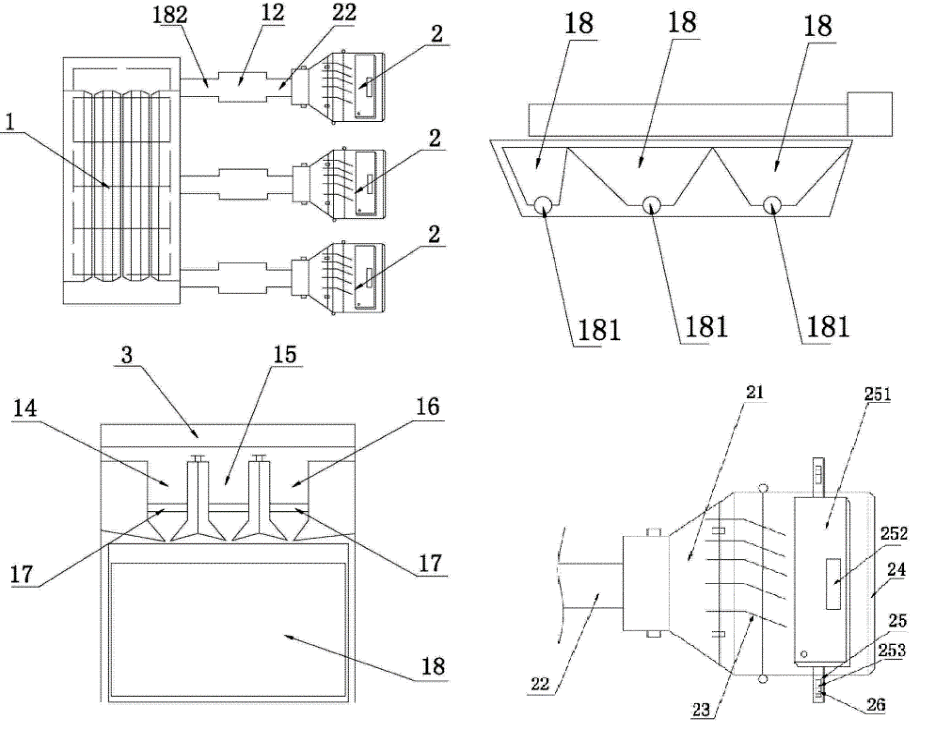
\includegraphics[width=1\textwidth]{chapter1/clasificador y contador de peces de origen chino.png}
	\caption{Clasificadora automática de peces de origen chino.}
	Fuente: Patente CN203884438U.
	\label{fig:clasificador y contador de peces de origen chino}
\end{figure}

%% NUEVA SUB-SUB-SECCION X.X.X.X
\subsubsection{Seleccionadora completamente automática \textit{AGK}}

Según el fabricante, las ventajas de este sistema son la suavidad y principios de ajuste simples, construcción ligera, freno automático, suministro de agua simple, buena estabilidad, embudo de llenado extraíble. En cuanto a la clasificación: puede ser usada en truchas de 8 a 10, 10 a 20 y de 20 a 30 centímetros como rangos para clasificación. Las dimensiones de la seleccionadora son de 3500x1000x1180 milímetros. El peso de la máquina es de 150 kilogramos y tiene una potencia de 0.15 kW ya que hace uso cintas transportadoras y admite un suministro eléctrico de 220 y 380 VAC. Los materiales usados en la clasificadora son de acero galvanizado, acero inoxidable, aluminio y plástico.\citep{AGKAquakultur-Teich2010} Sin embargo, el fabricante menciona que la venta es solo para medianas y grandes empresas, según la normativa alemana.

\begin{figure}[H]
	\centering
	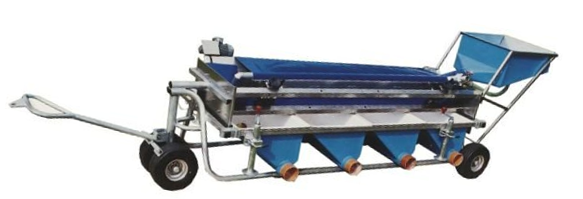
\includegraphics[width=1\textwidth]{chapter1/clasificadora de peces de origen aleman.png}
	\caption{Clasificadora de peces de origen alemán.}
	Fuente: AGK – Aquakultur-Teich.
	\label{fig:clasificadora de peces de origen aleman}
\end{figure}

%% NUEVA SUB-SUB-SECCION X.X.X.X
\subsubsection{Clasificador automático para peces \textit{Helios}}
\label{sssec:clasificador automatico para peces helios}

La empresa FAIVRE comercializa la máquina clasificadora Helios 25 para truchas de 5 a 350 gramos (Figura \ref{fig:clasificadoras automaticas para peces de origen frances}) con capacidad para clasificar en 3 tamaños con 2 rieles de clasificación. La máquina está hecha de acero inoxidable AISI 304L o 316L de alta calidad \citep[p.~1]{FAIVRE2019a}. El funcionamiento se divide en tres etapas: primero el sistema de recepción y canalización recibe los peces mediante la conexión a una bomba de peces en funcionamiento y los envía al siguiente sistema de manera que no ingresen dos peces al mismo tiempo; segundo, los peces pasan por canales (Figura \ref{fig:sistema de canalizacion de peces}) impulsados por cadenas transportadoras en los laterales que poseen tiras de goma para trasladar hasta que se clasifique mecánicamente; tercero, luego de estar en la sección respectiva la trucha sale de la máquina mediante tuberías.

\begin{figure}[H]
	\centering
	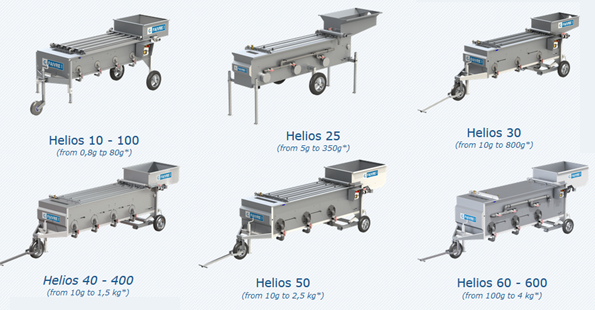
\includegraphics[width=1\textwidth]{chapter1/clasificadoras automaticas para peces de origen frances.png}
	\caption{Clasificadoras automáticas para peces de origen francés.}
	Fuente: Empresa acuícola FAIVRE.
	\label{fig:clasificadoras automaticas para peces de origen frances}
\end{figure}

\begin{figure}[H]
	\centering
	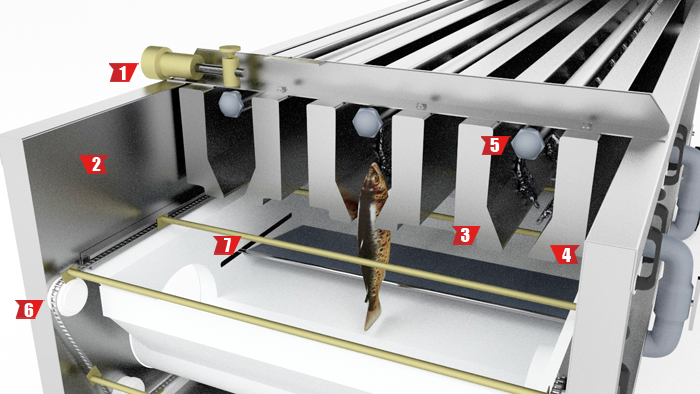
\includegraphics[width=1\textwidth]{chapter1/sistema de canalizacion de peces.png}
	\caption{Clasificadoras automáticas para peces de origen francés.}
	1. Configuración - 2. Panel lateral - 3. Panel ajustable - 4. Panel fijo \\
	5. Riego - 6. Cadena transportadora - 7. Tiras de goma\\
	Fuente: \citep{FAIVRE2018}.
	\label{fig:sistema de canalizacion de peces}
\end{figure}

La empresa francesa cuenta con máquinas que pueden clasificar y posteriormente contar para saber la cantidad de peces que se están redistribuyendo como se visualiza en la Figura \ref{fig:seleccionador con contador integrado y sus partes}. En esta versión además incluye una interfaz de control más avanzada con más funciones.

\begin{figure}[H]
	\centering
	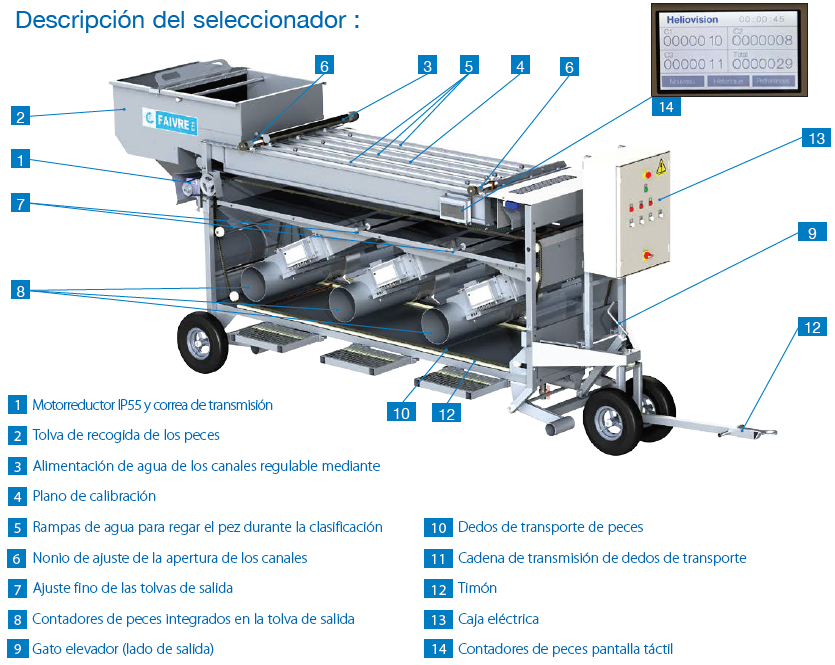
\includegraphics[width=1\textwidth]{chapter1/seleccionador con contador integrado y sus partes.png}
	\caption{Seleccionador con contador integrado y sus partes.}
	Fuente: FAIVRE.
	\label{fig:seleccionador con contador integrado y sus partes}
\end{figure}

%% NUEVA SUB-SUB-SECCION X.X.X.X
\subsubsection{Clasificador automático de peces y contador automático \textit{Pentair V-100 00140}}

Pentair se dedica al diseño y venta de máquinas acuícolas a pedido. La cotización de una clasificadora (\textit{Pentair V-100 00140}) y contadora (\textit{Pentair V-10007}) muestra precios elevados como se muestra en la Tabla \ref{tbl:extracto de cotizacion de maquinas clasificadora y contadora para peces}. El diseñador y fabricante asegura tener una cercana a 97\%. La cotización implicó brindar datos: el estándar de suministro eléctrico peruano, el tipo de pez a contar (\textit{trucha}), el rango de gramajes y la dirección de destino. Además, Pentair especificó que las máquinas cotizadas funcionan como un sistema unido y que, si se empleaba otras marcas en ese sistema, la marca no se responsabilizaba por mal funcionamiento.

% Please add the following required packages to your document preamble:
% \usepackage[table,xcdraw]{xcolor}
% If you use beamer only pass "xcolor=table" option, i.e. \documentclass[xcolor=table]{beamer}
\begin{table}[H]
	\centering
	\caption{Extracto de cotización de máquinas clasificadora y contadora para peces.}
	\label{tbl:extracto de cotizacion de maquinas clasificadora y contadora para peces}
	\begin{tabular}{|l|l|l|r|r|l|r|r|}
		\hline
		\rowcolor[HTML]{A6A6A6} 
		\multicolumn{1}{|c|}{\cellcolor[HTML]{A6A6A6}{\color[HTML]{000000} \textbf{N°}}} &
		\multicolumn{1}{c|}{\cellcolor[HTML]{A6A6A6}{\color[HTML]{000000} \textbf{Ítem}}} &
		\multicolumn{1}{c|}{\cellcolor[HTML]{A6A6A6}{\color[HTML]{000000} \textbf{\rot{Detalles}}}} &
		\multicolumn{1}{c|}{\cellcolor[HTML]{A6A6A6}{\color[HTML]{000000} \textbf{\rot{Cantidad}}}} &
		\multicolumn{1}{c|}{\cellcolor[HTML]{A6A6A6}{\color[HTML]{000000} \textbf{\rot{Acordado}}}} &
		\multicolumn{1}{c|}{\cellcolor[HTML]{A6A6A6}{\color[HTML]{000000} \textbf{\rot{UM}}}} &
		\multicolumn{1}{c|}{\cellcolor[HTML]{A6A6A6}{\color[HTML]{000000} \textbf{\rot{Precio unitario}}}} &
		\multicolumn{1}{c|}{\cellcolor[HTML]{A6A6A6}{\color[HTML]{000000} \textbf{\rot{Precio total (\$)}}}} \\ \hline
		2 &
		\begin{tabular}[c]{@{}l@{}}V-10007\\ MACRO COUNTER,\\ THREE/FOUR CHANNEL\\ Vaki Macro 4 channel counter \\ for fish from 0.2g up to 400g.\\ Counts graded fish in up to\\ 4 channels simultaneously.\end{tabular} &
		- &
		1.0 &
		1.0 &
		EA &
		64 027.00 &
		64 027.00 \\ \hline
		3 &
		\begin{tabular}[c]{@{}l@{}}V-100 00140\\ GRADER 140CM DIAMETER\\ Vaki 140cm rotary fish grader. \\ Grades fish from 0.5g up to \\ 200g in up to grades. Includes \\ dewatering system and spray bar.\end{tabular} &
		- &
		1.0 &
		1.0 &
		EA &
		53 567.00 &
		53 567.00 \\ \hline
	\end{tabular}
\\ Fuente: Pentair.
\end{table}

%% NUEVA SUB-SUB-SECCION X.X.X.X
\subsubsection{Clasificador de peces \textit{Apollo}}

Este tipo de clasificador suele ser destinado al uso industrial. El fabricante tiene diferentes máquinas con diferentes gramajes para clasificar (\textit{1 a 650 g y 5 a 750 g}). Tiene cuatro de tres a cuatro salidas. Usa el suministro eléctrico estándar noruego (\textit{230/400 VAC 50Hz.}). Realiza el conteo de hasta cuatro toneladas por hora cuando clasifica salmones de un rango específico (\textit{300 a 400 g}). El sistema clasifica de forma similar al representado en la Figura REF. \citep{Apollo2013}

\begin{figure}[H]
	\centering
	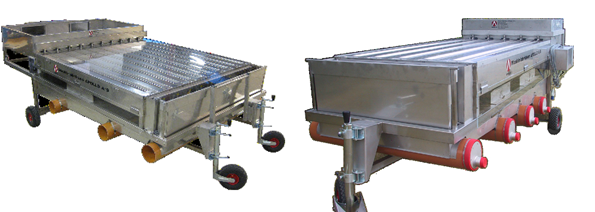
\includegraphics[width=1\textwidth]{chapter1/clasificadora de peces de origen danes.png}
	\caption{Clasificadora de peces de origen danés.}
	Fuente: \citep{Apollo2013}
	\label{fig:clasificadora de peces de origen danes}
\end{figure}

%% NUEVA SUB-SUB-SECCION X.X.X.X
\subsubsection{Contador de peces \textit{Pescavision}}

Los contadores de peces mostrados en la Figura \ref{fig:contador pescavision 100 300 10x4} funcionan bajo el mismo principio que sus clasificadores mostrados en incisos anteriores, es decir, mediante el uso de barreras de luz infrarroja. El fabricante asegura que los modelos \textit{Pescavision50} y \textit{Pescavision300} pueden llegar a tener una precisión total (\textit{100\%}) y conforme aumenta sus capacidades de conteo aumenta también las dimensiones de la máquina y el gramaje mínimo que puede contar. A diferencia de otros sistemas estas máquinas sí son compatibles con el estándar de electricidad que se emplea en Perú.

\begin{figure}[H]
	\centering
	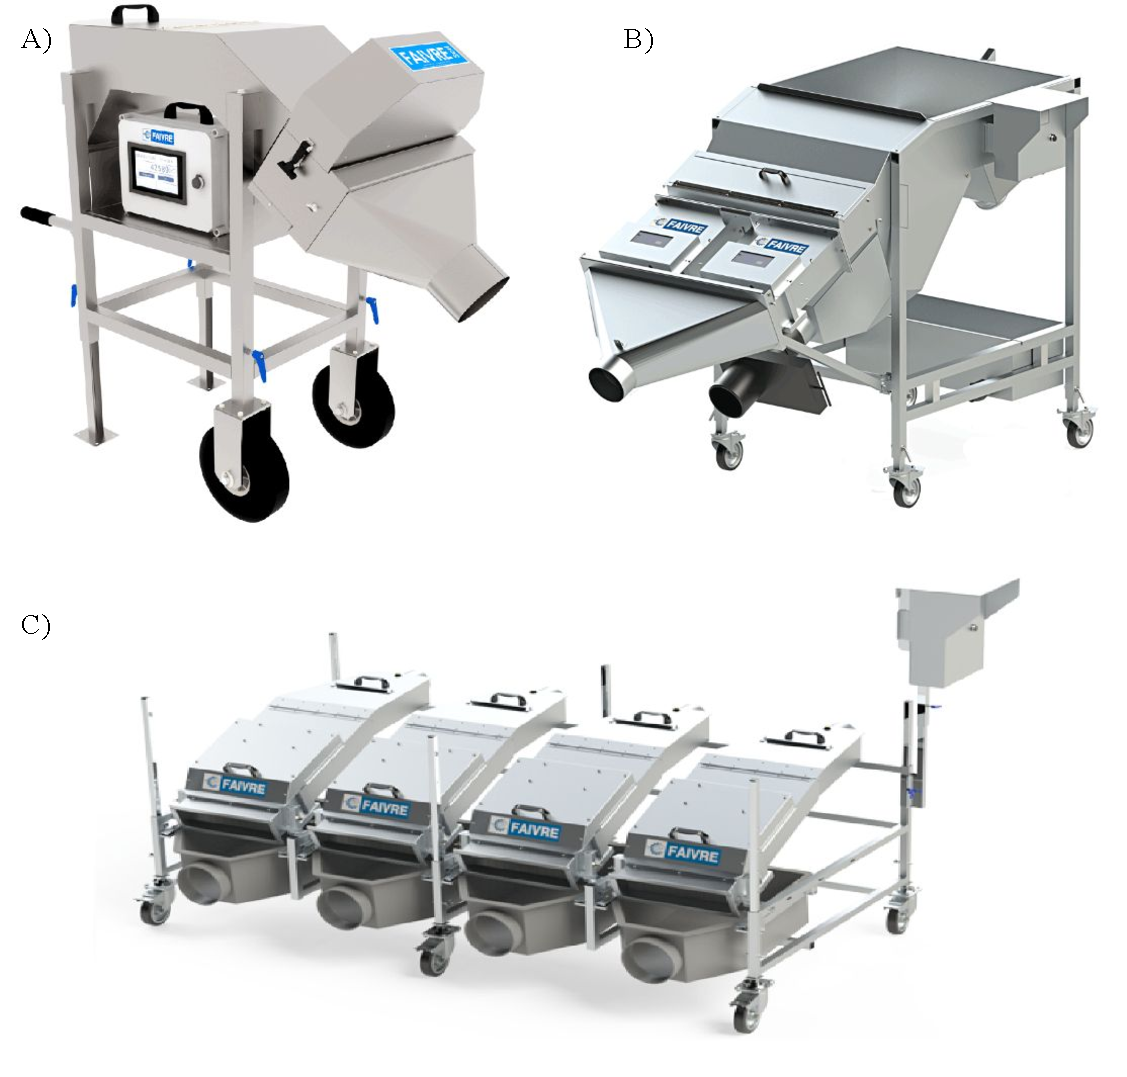
\includegraphics[width=1\textwidth]{chapter1/contador pescavision 100 300 10x4.pdf}
	\caption{(a,b,c)  Contador Pescavision 100, Pescavision 300 y Pescavision 10x4.}
	Fuente: \citep{FAIVRE2019a}
	\label{fig:contador pescavision 100 300 10x4}
\end{figure}

%% NUEVA SUB-SUB-SECCION X.X.X.X
\subsubsection{Contador de peces \textit{Calitri}}

El contador de peces Calitri funciona tanto en agua dulce como salada, está diseñado para brindar una precisión del 97\% al momento de contar los peces, cuenta con di-versos modelos con diferentes números de canales de conteo (\textit{2, 4, 8 y 12 canales}). La máquina puede recibir los peces de forma manual mediante la adaptación de una tolva a su entrada.\citep{Calitri2018} Según el fabricante, el conteo se realiza mediante sensores que captan una señal que si es bloqueada en momentos significa que hay un pez en medio.

\begin{figure}[H]
	\centering
	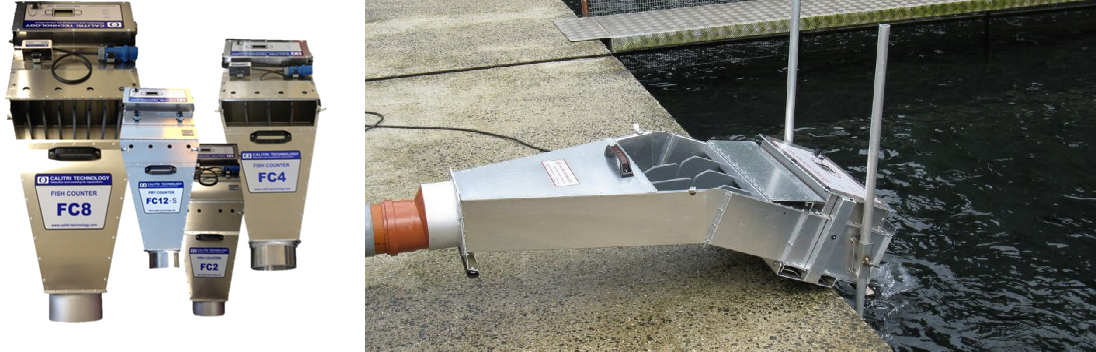
\includegraphics[width=1\textwidth]{chapter1/contador de peces de origen belga.png}
	\caption{Contador de peces de origen belga.}
	Fuente: Calitri Technology.
	\label{fig:contador de peces de origen belga}
\end{figure}

%% NUEVA SUB-SUB-SECCION X.X.X.X
\subsubsection{Comparación}

En la Tabla \ref{tbl:comparacion de clasificadores comerciales} se muestra la comparación entre máquinas clasificadoras\footnote{También llamadas seleccionadoras.}. El análisis para realizar esta comparación fue de forma cuantitativa y cualitativa a juicio del autor de este trabajo. La \textbf{compra} se refiere a la forma de adquisición del producto. El \textbf{rango} se refiere a los límites inferior y superior que la máquina asegura poder clasificar. Las \textbf{entradas} se refieren al número de sistemas de recepción de la máquina y \textbf{salidas} se refieren a la cantidad de rangos clasificados. La \textbf{capacidad por hora} es la cantidad máxima de peces que se pueden clasificar cada hora. El \textbf{suministro eléctrico} es la tensión eléctrica estándar que necesita, los productos internacionales usan diferentes niveles de tensión y frecuencia.  La mínima \textbf{velocidad de entrada del caudal} es la velocidad mínima para que el sistema pueda clasificar correctamente. La \textbf{precisión} se calcula como la cantidad de peces correctamente clasificados dividido con la cantidad de peces incorrectamente clasificados. El \textbf{precio} no incluye cargos por envío o de impuestos.

% Please add the following required packages to your document preamble:
% \usepackage[table,xcdraw]{xcolor}
% If you use beamer only pass "xcolor=table" option, i.e. \documentclass[xcolor=table]{beamer}
\begin{savenotes}
	\begin{table}[H]
		\centering
		\caption{Comparación de clasificadores comerciales.}
		\label{tbl:comparacion de clasificadores comerciales}
		\begin{tabular}{|
			>{\columncolor[HTML]{D9D9D9}}l |c|c|c|c|}
			\hline
			\multicolumn{1}{|c|}{\cellcolor[HTML]{A6A6A6}{\color[HTML]{000000} \textbf{Criterio\textbackslash{}Método}}} &
			\cellcolor[HTML]{A6A6A6}{\color[HTML]{000000} \textbf{AGK}} &
			\cellcolor[HTML]{A6A6A6}{\color[HTML]{000000} \textbf{HELIOS 25\footnote{También existe Helios 10, 30, 40, 50, 60 y 100. En el Anexo A2 se muestra las características de cada una.}}} &
			\cellcolor[HTML]{A6A6A6}{\color[HTML]{000000} \textbf{APOLLO}} &
			\cellcolor[HTML]{A6A6A6}{\color[HTML]{000000} \textbf{\begin{tabular}[c]{@{}c@{}}PENTAIR\\ V-10000140\footnote{Cotización a empresa Pentair en el Anexo A3.}\end{tabular}}} \\ \hline
			{\color[HTML]{000000} Compra} &
			{\color[HTML]{000000} \begin{tabular}[c]{@{}c@{}}Depende\\ del stock\end{tabular}} &
			{\color[HTML]{000000} \begin{tabular}[c]{@{}c@{}}Depende\\ del stock\end{tabular}} &
			{\color[HTML]{000000} \begin{tabular}[c]{@{}c@{}}Depende\\ del stock\end{tabular}} &
			{\color[HTML]{000000} A pedido\footnote{Diseño y envío de 6 a 8 semanas luego de ordenar y realizar el pago. Las especificaciones se indican luego de diseñado el producto.}} \\ \hline
			{\color[HTML]{000000} Rango ($ g $)} &
			{\color[HTML]{000000} 10 a 200} &
			{\color[HTML]{000000} 5 a 400} &
			{\color[HTML]{000000} \begin{tabular}[c]{@{}c@{}}1 a 650\\ 5 a 750\end{tabular}} &
			{\color[HTML]{000000} 0.5 a 200} \\ \hline
			{\color[HTML]{000000} Entradas} &
			{\color[HTML]{000000} 1} &
			{\color[HTML]{000000} 1} &
			{\color[HTML]{000000} 1} &
			{\color[HTML]{000000} 1} \\ \hline
			{\color[HTML]{000000} Salidas} &
			{\color[HTML]{000000} 4} &
			{\color[HTML]{000000} 6} &
			{\color[HTML]{000000} 4} &
			{\color[HTML]{000000} -} \\ \hline
			{\color[HTML]{000000} Capacidad por hora} &
			{\color[HTML]{000000} 70 000} &
			{\color[HTML]{000000} 95 000} &
			{\color[HTML]{000000} 95 000} &
			{\color[HTML]{000000} -} \\ \hline
			{\color[HTML]{000000} Potencia} &
			{\color[HTML]{000000} 0.15 kW} &
			{\color[HTML]{000000} 0.37 kW} &
			{\color[HTML]{000000} 0.18 kW} &
			{\color[HTML]{000000} -} \\ \hline
			{\color[HTML]{000000} RPM} &
			{\color[HTML]{000000} -} &
			{\color[HTML]{000000} -} &
			{\color[HTML]{000000} 900} &
			{\color[HTML]{000000} -} \\ \hline
			{\color[HTML]{000000} \begin{tabular}[c]{@{}l@{}}Suministro eléctrico\\ ($ V-Hz. $)\end{tabular}} &
			{\color[HTML]{000000} \begin{tabular}[c]{@{}c@{}}220/380   VAC \\ 50/60   Hz.\end{tabular}} &
			{\color[HTML]{000000} \begin{tabular}[c]{@{}c@{}}230   VAC\\ 50/60   Hz.\end{tabular}} &
			{\color[HTML]{000000} \begin{tabular}[c]{@{}c@{}}230/400\\ VAC  50 Hz.\end{tabular}} &
			{\color[HTML]{000000} \begin{tabular}[c]{@{}c@{}}220/230\\ VAC 60 Hz.\end{tabular}} \\ \hline
			{\color[HTML]{000000} Recepción de peces} &
			{\color[HTML]{000000} \begin{tabular}[c]{@{}c@{}}Manual /\\ Bombeo\\de peces\end{tabular}} &
			{\color[HTML]{000000} \begin{tabular}[c]{@{}c@{}}Manual /\\  Bombeo\\de peces\end{tabular}} &
			{\color[HTML]{000000} \begin{tabular}[c]{@{}c@{}}Manual /\\ Bombeo\\de peces\end{tabular}} &
			{\color[HTML]{000000} \begin{tabular}[c]{@{}c@{}}Bombeo\\ de peces\end{tabular}} \\ \hline
			{\color[HTML]{000000} \begin{tabular}[c]{@{}l@{}}Mínima velocidad de \\ entrada de caudal ($ m^3/h $)\end{tabular}} &
			{\color[HTML]{000000} -} &
			{\color[HTML]{000000} 40} &
			{\color[HTML]{000000} \begin{tabular}[c]{@{}c@{}}Bombeo\\de peces\end{tabular}} &
			{\color[HTML]{000000} -} \\ \hline
			{\color[HTML]{000000} Dimensiones ($ cm $)\footnote{Las dimensiones de la máquina son de largo($ l $), ancho($ a $) y alto($ h $).}} &
			{\color[HTML]{000000} 350x100x118} &
			{\color[HTML]{000000} 200x100x110\footnote{Altura ajustable de 110 a 140 $ cm $.}} &
			{\color[HTML]{000000} 315x128x128\footnote{Altura ajustable de 128 a 145 $ cm $.}} &
			{\color[HTML]{000000} -} \\ \hline
			{\color[HTML]{000000} Peso ($ kg $)} &
			{\color[HTML]{000000} 150} &
			{\color[HTML]{000000} 210} &
			{\color[HTML]{000000} 375} &
			{\color[HTML]{000000} -} \\ \hline
			{\color[HTML]{000000} Precisión ($ \% $)} &
			{\color[HTML]{000000} -} &
			{\color[HTML]{000000} 97} &
			{\color[HTML]{000000} -} &
			{\color[HTML]{000000} 97} \\ \hline
			{\color[HTML]{000000} Precio ($ \$ $)} &
			{\color[HTML]{000000} -} &
			{\color[HTML]{000000} -} &
			{\color[HTML]{000000} 15 730} &
			{\color[HTML]{000000} 53 567} \\ \hline
		\end{tabular}
	\\Fuente: AGK, Helios 25, Apollo, Pentair y Elaboración propia.
	\end{table}
\end{savenotes}

En la Tabla \ref{tab:comparacion de contadores comerciales} se resume la comparación entre contadores de truchas comerciales El análisis para realizar esta comparación fue de forma cuantitativa y cualitativa a juicio del autor de este trabajo. 

% Please add the following required packages to your document preamble:
% \usepackage[table,xcdraw]{xcolor}
% If you use beamer only pass "xcolor=table" option, i.e. \documentclass[xcolor=table]{beamer}
\begin{savenotes}
	\begin{table}[H]
		\centering
		\caption{Comparación de contadores comerciales.}
		\label{tab:comparacion de contadores comerciales}
		\begin{tabular}{|
				>{\columncolor[HTML]{D9D9D9}}l |c|c|c|c|}
			\hline
			\multicolumn{1}{|c|}{\cellcolor[HTML]{A6A6A6}{\color[HTML]{000000} \textbf{Criterio\textbackslash{}Método}}} &
			\cellcolor[HTML]{A6A6A6}{\color[HTML]{000000} \textbf{\begin{tabular}[c]{@{}c@{}}CALITRI \\ FC4\end{tabular}}} &
			\cellcolor[HTML]{A6A6A6}{\color[HTML]{000000} \textbf{\begin{tabular}[c]{@{}c@{}}PESCAVISION\\ 50\footnote{Folleto en el Anexo A2.}\end{tabular}}} &
			\cellcolor[HTML]{A6A6A6}{\color[HTML]{000000} \textbf{\begin{tabular}[c]{@{}c@{}}PESCAVISION\\ 300\footnote{Folleto en el Anexo A2.}\end{tabular}}} &
			\cellcolor[HTML]{A6A6A6}{\color[HTML]{000000} \textbf{\begin{tabular}[c]{@{}c@{}}PENTAIR\\ V-10007\footnote{Cotización a empresa Pentair en el Anexo A3.}\end{tabular}}} \\ \hline
			{\color[HTML]{000000} Compra} &
			{\color[HTML]{000000} \begin{tabular}[c]{@{}c@{}}Depende\\ del stock\end{tabular}} &
			{\color[HTML]{000000} \begin{tabular}[c]{@{}c@{}}Depende\\ del stock\end{tabular}} &
			{\color[HTML]{000000} \begin{tabular}[c]{@{}c@{}}Depende\\ del stock\end{tabular}} &
			{\color[HTML]{000000} A pedido} \\ \hline
			{\color[HTML]{000000} Rango ($ g $)} &
			{\color[HTML]{000000} 50 a 900} &
			{\color[HTML]{000000} 5 a 4500} &
			{\color[HTML]{000000} 40 a 1000} &
			{\color[HTML]{000000} 0.2 a 4000} \\ \hline
			{\color[HTML]{000000} Canales de conteo} &
			{\color[HTML]{000000} 4} &
			{\color[HTML]{000000} 2} &
			{\color[HTML]{000000} 8} &
			{\color[HTML]{000000} 4} \\ \hline
			{\color[HTML]{000000} Capacidad por hora} &
			{\color[HTML]{000000} 95 000} &
			{\color[HTML]{000000} 95 000} &
			{\color[HTML]{000000} 165 000} &
			{\color[HTML]{000000} -} \\ \hline
			{\color[HTML]{000000} \begin{tabular}[c]{@{}l@{}}Suministro eléctrico\\ ($ V-Hz. $)\end{tabular}} &
			{\color[HTML]{000000} \begin{tabular}[c]{@{}c@{}}90/220   VAC \\ 50/60   Hz.\end{tabular}} &
			{\color[HTML]{000000} \begin{tabular}[c]{@{}c@{}}220 VAC 50/60\\ Hz. / 24 VDC\end{tabular}} &
			{\color[HTML]{000000} \begin{tabular}[c]{@{}c@{}}220 VAC\\ 50-60 Hz.\end{tabular}} &
			{\color[HTML]{000000} \begin{tabular}[c]{@{}c@{}}220/230\\ VAC 60 Hz.\end{tabular}} \\ \hline
			{\color[HTML]{000000} Recepción de peces} &
			{\color[HTML]{000000} \begin{tabular}[c]{@{}c@{}}Manual / \\ Bombeo \\ de peces\end{tabular}} &
			{\color[HTML]{000000} \begin{tabular}[c]{@{}c@{}}Sistema de\\  clasificación \\ FAIVRE\end{tabular}} &
			{\color[HTML]{000000} \begin{tabular}[c]{@{}c@{}}Sistema de \\ clasificación \\ FAIVRE\end{tabular}} &
			{\color[HTML]{000000} \begin{tabular}[c]{@{}c@{}}Bombeo \\ de peces\end{tabular}} \\ \hline
			{\color[HTML]{000000} \begin{tabular}[c]{@{}l@{}}Mínima velocidad de \\ entrada de caudal ($ m^3/h $)\end{tabular}} &
			{\color[HTML]{000000} 12} &
			{\color[HTML]{000000} 40} &
			{\color[HTML]{000000} 40} &
			{\color[HTML]{000000} 40} \\ \hline
			{\color[HTML]{000000} Dimensiones ($ cm $)\footnote{Las dimensiones de la máquina son de largo($ l $),
					 ancho($ a $) y alto($ h $).}} &
			{\color[HTML]{000000} 125x50x35} &
			{\color[HTML]{000000} 150x50x60} &
			{\color[HTML]{000000} 200x150x100} &
			{\color[HTML]{000000} -} \\ \hline
			{\color[HTML]{000000} Peso ($ kg $)} &
			{\color[HTML]{000000} 18} &
			{\color[HTML]{000000} 20} &
			{\color[HTML]{000000} 375} &
			{\color[HTML]{000000} -} \\ \hline
			{\color[HTML]{000000} Precisión ($ \% $)} &
			{\color[HTML]{000000} 97} &
			{\color[HTML]{000000} 98-100} &
			{\color[HTML]{000000} 98-100} &
			{\color[HTML]{000000} 97} \\ \hline
			{\color[HTML]{000000} Precio ($ \$ $)} &
			{\color[HTML]{000000} 5 705.37} &
			{\color[HTML]{000000} -} &
			{\color[HTML]{000000} -} &
			{\color[HTML]{000000} 64 027.00} \\ \hline
		\end{tabular}
	\\ Fuente: Calitri, FAIVRE, Pentair y Elaboración propia.
	\end{table}
\end{savenotes}


%% Contenido
%\begin{spacing}{1.5}
%{Ejemplo de cuerpo y ejemplo de imagen en l \ref{fig:PLACEHOLDER}. }
%\begin{equation} \label{eq:1}
%    S=\sum_iP_ilog(P_i)
%\end{equation}
%\end{spacing}
%% Fin de contenido